% Edubot
% Diplomarbeit HTL-Grieskirchen
% Schuljahr 2011/12 
%
% diplomarbeit.tex: Hauptdatei der Diplomarbeit
% Autoren: Philipp Stelzer, David Maier



\documentclass[pdftex, 
			   a4paper, 
			   12pt, lequo, 
			   final]{scrartcl}
\usepackage[style=footnote-dw, autocite=footnote]{biblatex}
\usepackage[german]{babel}
\usepackage[utf8]{inputenc}
\usepackage[T1]{fontenc}
\usepackage{listings}
\usepackage{graphicx}
\usepackage{fancyhdr}
\usepackage{titlesec}
\usepackage{subfigure}
\usepackage{setspace}
\usepackage{listing}
\usepackage{listingsutf8}
\usepackage{color} 
\usepackage{colortbl}
\definecolor{gray}{rgb}{0.4,0.4,0.4} 
\definecolor{lightgray}{rgb}{0.95,0.95,0.95}
\definecolor{darkred}{rgb}{0.6,0.0,0.0} 
\definecolor{red}{rgb}{1.0,0.0,0.0} 
\definecolor{blue}{rgb}{0.0,0.0,1.0} 
\definecolor{darkblue}{rgb}{0.0,0.0,0.6} 
\definecolor{cyan}{rgb}{0.0,0.6,0.6}
\usepackage{color}
\usepackage{float}
\usepackage{array, ragged2e}
\usepackage{caption}
\usepackage{longtable}
\usepackage{beramono}
\usepackage{url}
\usepackage{eurosym}
\usepackage{geometry}
\usepackage{amsmath}
\usepackage[pdftex,
            pdfauthor={Philipp Stelzer \& David Maier},
            pdftitle={Edubot},
            pdfsubject={Diplomarbeit aus Prozessregelung mit Laborübungen},
            pdfproducer={LaTeX},
            pdfcreator={PDFLaTeX}]{hyperref}
\renewcommand{\familydefault}{\sfdefault}
\geometry{a4paper, left=3cm, right=3cm, top=2.5cm, bottom=2.5cm}
\bibliography{misc/references}

\definecolor{pink}{rgb}{1,.21,.86}

\lstset{
  basicstyle=\ttfamily,
  columns=fullflexible,
  showstringspaces=false,
  breaklines=true,
  commentstyle=\color{0.133,0.545,0.133}\upshape
}

\lstdefinelanguage{XAML}
{
  morestring=[b]",
  morestring=[b]{>}{<},
  morecomment=[s]{<?}{?>},
  stringstyle=\color{blue},
  identifierstyle=\color{darkred},
  keywordstyle=\color{red},
  morekeywords={xmlns,version,type,Grid.Row, Grid.Column, Margin, Width, Height, HorizontalAlignment, VerticalAlignment, IsEnabled, Name, Path, UpdateSourceTrigger}% list your attributes here
} 

\lstdefinelanguage{codesysls}
{
	sensitive=true,
morekeywords=[1]{ ,
CASE, OF, IF, END_IF, ELSIF, THEN, END_CASE, AND, OR, VAR, VAR_IN, DINT, INT, LREAL, PROGRAMM, END_VAR, FUNCTION, FUNCTION_BLOCK},
morekeywords=[2]{,TRUE,FALSE},
keywordstyle=[1]\color{blue},
keywordstyle=[2]\color{pink},
morecomment=[s]{(*}{*)},
}

\lstdefinelanguage{CSharp}
{
  sensitive=true,
morekeywords=[1]{ ,
abstract, as, base, break, case,
catch, checked, class, const, continue,
default, delegate, do, else, enum,
event, explicit, extern, false,
finally, fixed, for, foreach, goto, if,
implicit, in, interface, internal, is,
lock, namespace, new, null, operator,
out, override, params, private,
protected, public, readonly, ref,
return, sealed, sizeof, stackalloc,
static, struct, switch, this, throw,
true, try, typeof, unchecked, unsafe,
using, virtual, volatile, while, bool,
byte, char, decimal, double, float,
int, lock, object, sbyte, short, string,
uint, ulong, ushort, void},
morekeywords=[2]{,ICommand, AbortCommand, StartCommand, ShutdownCommand, MVSCommand, MVCCommand, UseToolCommand, IAdapter, EdubotAdapter, VirtualAdapter, Cursors, FileStream, XmlSerializer, UnauthorizedAccessException, FileMode, MessageBox, MessageBoxButton, MessageBoxImage, Point3D, Math, MathHelper, Event, EventArgs, HomingEventArgs, MovementStartedEventArgs, ToolUsedEventArgs, FailureEventArgs, StateChangedEventArgs, List, ThreadAbortException, State, KeyValuePair, StrokeCollection, Memento, InkCanvasStrokeCollectedEventArgs, StylusPoint, StylusPointCollection, Point, InterpolationType, Path,}
keywordstyle=[1]\color{blue},
keywordstyle=[2]\color{cyan},
morecomment=[l]{//},
morecomment=[s]{/*}{*/},
morestring=[b]",
morestring=[b]'
}

%Bibliography Style
\DeclareBibliographyDriver{misc}{%
  \usebibmacro{bibindex}%
  \usebibmacro{begentry}%
  %\printtext{\printnames{labelname}}
  \usebibmacro{author/editor+others/translator+others}%
  \setunit{\labelnamepunct}\newblock
  \usebibmacro{title}%
  \setunit{. }\newblock
  \printfield{year}%
  \setunit{. }\newblock
  \printfield{note}%
  \newunit\newblock
  \usebibmacro{doi+eprint+url}%
  \newunit\newblock
  \usebibmacro{addendum+pubstate}%
  \setunit{\bibpagerefpunct}\newblock
  \usebibmacro{pageref}%
  \usebibmacro{finentry}}

\DeclareBibliographyDriver{book}{%
  \usebibmacro{bibindex}%
  \usebibmacro{begentry}%
  \usebibmacro{author/editor+others/translator+others}%
  \setunit{\labelnamepunct}\newblock
  \usebibmacro{maintitle+title}%
  \setunit{. - }\newblock
  \printlist{location}%
  \setunit{\labelnamepunct}\newblock
  \printlist{publisher}
  \printfield{year}%
  \printtext{. }
  \newunit\newblock
  \usebibmacro{chapter+pages}%
  \newunit
  \printfield{pagetotal}%
  \newunit\newblock
  \iftoggle{bbx:isbn}
    {\printfield{isbn}}
    {}%
  \newunit\newblock
  \usebibmacro{doi+eprint+url}%
  \newunit\newblock
  \usebibmacro{addendum+pubstate}%
  \setunit{\bibpagerefpunct}\newblock
  \usebibmacro{pageref}%
  \usebibmacro{finentry}}
  
  \newbibmacro*{cite}{% 
  	\ifciteseen{
    	   \printtext{\printnames{labelname} \printfield{year}}
       }{
       \printtext{% 
          \usedriver 
          {\DeclareNameAlias{default}{sortname}} 
          {\thefield{entrytype}}}% 
       }}



%pdf metatags

%caption of pictures (skip)
\captionsetup{aboveskip=10pt}

%caption of figures
\renewcommand{\captionfont}{\small}

\newcommand{\titleformatsection}[1]
		   {\titleformat{\section}
		   {\normalfont\LARGE\bfseries}
		   {\thesection}{1em}{#1}}
\newcommand{\titleformatsubsection}[1]
		   {\titleformat{\subsection}
		   {\normalfont\Large\bfseries}
		   {\thesubsection}{1em}{#1}}
\newcommand{\titleformatsubsubsection}[1]
		   {\titleformat{\subsubsection}
		   {\normalfont\large\bfseries}
		   {\thesubsubsection}{1em}{#1}}
		   
\titleformat{\paragraph}[hang]{\normalfont\bfseries}{}{0pt}{}
\titleformat{\subparagraph}[hang]{\normalfont\bfseries}{}{0pt}{}
\titlespacing{\paragraph}{0mm}{5pt}{4pt}
\titlespacing{\subparagraph}{0mm}{3pt}{2pt}

\newenvironment{myitemize}
			   {\begin{itemize}\itemsep0.0pt\parskip1.0ex}
			   {\end{itemize}\parskip1.5ex}
			   
\newcolumntype{C}[1]{>{\Centering}m{#1}}

%setting up the code listings
\definecolor{listinggray}{gray}{0.9}
\definecolor{lightblue}{rgb}{0.0,0.0,0.5}
\definecolor{lightgreen}{rgb}{0.0,0.5,0.0}
\lstset{numbers=left}
\lstset{numberstyle=\footnotesize\ttfamily}
\lstset{numbersep=5pt} 
\lstset{language=[SHARP]C}
\lstset{backgroundcolor=\color{listinggray}}
\lstset{basicstyle=\footnotesize\ttfamily}
\lstset{keywordstyle=\color{lightblue}}
\lstset{commentstyle=\color{blue}}
\lstset{stringstyle=\color{lightgreen}}
\lstset{morecomment=[s][\color{blue}]{/*}{*/}}




%say latex that listings are atomar
\newfloat{makeatomar}{tp}{lot}[section]

%!!! IMPORTANT FOR TEXT FLOW !!!
\raggedbottom

%\setlength{\evensidemargin}{0.76cm}
%\setlength{\oddsidemargin}{-0.54cm}
	
\parskip1.5ex
\parindent0.0ex
%
% EoF
%

\begin{document}
	\pagestyle{empty}
	
\begin{titlepage}

	\begin{figure}[H]
	\hspace{10cm}
		
\includegraphics[width=6cm]{images/htl_logo}
	\end{figure}
	\vspace*{3cm}
	
	\begin{center}
		\Huge
		HTL der Stadtgemeinde Grieskirchen\\
		\vspace{0.5cm}
		\Large
		Fachrichtung EDV und Organisation\\
		\vspace{0.5cm}
		\large
		Partzer Schulstraße 1, 4710 Grieskirchen
		\vspace{2cm}	
			
		\Huge
		\textbf{Edubot}\\
		\vspace{1cm}
		
		\large
		\textbf{Diplomarbeit}\\
		\textbf{von}\\
		\vspace{1em}
		Philipp Stelzer und David Maier\\
		\vspace{4cm}
		\normalsize
	\end{center}
	
	\hspace{2.85cm}
	\begin{tabular}{rl}
		\textbf{Fachgebiet:}   & PRRV 3\\
		\textbf{Betreuungslehrer:}   & Dipl.-Ing. Andreas Sperrer\\
		\textbf{Schuljahr:}   & 2011/12\\
		\textbf{Einreichungsdatum:}   & 14. Mai 2012\\
	\end{tabular}
	
	\normalsize
\end{titlepage}

%
% EoF
%

	
	\pagestyle{fancy}
	\fancyhf{}
	\renewcommand{\footrulewidth}{0.5pt}
	\renewcommand{\headrulewidth}{0.0pt}
	\onehalfspacing
	\fancyfoot[LO,RE]{\small \emph{Edubot - Roboter für Lehrzwecke}}
	\fancyfoot[RO,LE]{\small \thepage}
	\setlength{\footskip}{12mm}
	
	%  adjust the captions
	\titleformatsection{}
	\titleformatsubsection{}
	\titleformatsubsubsection{}
	
	\pagenumbering{Roman}
	
	
\phantomsection
\addcontentsline{toc}{section}{Eidesstattliche Erklärung}

\section*{Eidesstattliche Erklärung}

Ich erkläre an Eides statt, dass ich die vorliegende Diplomarbeit selbstständig und ohne fremde Hilfe verfasst, andere als die angegebenen Quellen und Hilfsmittel nicht benutzt und alle den benutzten Quellen wörtlich oder sinngemäß entnommenen Stellen als solche kenntlich gemacht habe.
%\\
\begin{flushleft}
	\footnotesize
	\begin{tabular}{@{}p{0.3\linewidth}p{0.1\linewidth}>{\centering\arraybackslash}p{0.5\linewidth}}
		& & \\ \cline{3-3} Grieskirchen, 11. Mai 2012 & & Philipp Stelzer \\ [2\baselineskip]
		& & \\ \cline{3-3} Grieskirchen, 11. Mai 2012 & & David Maier \\
	\end{tabular}
\end{flushleft}

%
% EoF
%

	\newpage
	
\phantomsection
\addcontentsline{toc}{section}{Abstract}

\section*{Abstract}
The target of the diploma project Edubot is the development of a simple-to-use, functional and effective tool for learning the operating principles of a robot. The outcome of this project will then be used in the subject "process control with laboratory exercises" during the “robotics” part of the third schoolyear. The diploma project includes the construction of a simple robot with two gyratory axes, an application programming interface (API) which enables the students to quickly and easily integrate the robot into their own programs, as well as an end-use application that can be used for presentation and teaching purposes. 

\section*{Kurzfassung}
Ziel der Diplomarbeit Edubot ist die Entwicklung eines einfach zu bedienenden, funktionellen und effektiven Werkzeugs zum Erlernen der Funktionsweise eines Roboters. Das Resultat dieses Projekts wird im Gegenstand "Prozessregelung mit Laborübungen" der 3. Klassen, im Zuge des Teilbereichs "Robotik" verwendet. Die Diplomarbeit beinhaltet die Konstruktion eines einfachen Roboters mit zwei rotatorischen Achsen, einer Anwendungsbibliothek (API) welche es den Schülern ermöglicht, den Roboter schnell und einfach ihre eigenen Programme zu integrieren, sowie eine Endanwendung welche zu Präsentations- und Lehrzwecken verwendet werden kann.


%
% EoF
%


	%
	% Table of Contents
	%
	\titleformatsection{\hfill}
	\clearpage
	\pagestyle{empty}
	\tableofcontents
	\clearpage
	\setcounter{page}{1}
		
	\pagestyle{fancy}
	\fancyfoot[LO,RE]{\small \emph{Edubot - Roboter für Lehrzwecke}}
	\fancyfoot[RO,LE]{\small \thepage}
	
	
	%
	% List of Figures
	%
	\newpage
	\setcounter{page}{3}
	\phantomsection
	\addcontentsline{toc}{section}{Abbildungsverzeichnis}
	\listoffigures
	
	
	%
	% List of Tables
	%
	%\newpage
	%\phantomsection
	%\addcontentsline{toc}{section}{Tabellenverzeichnis}
	%\listoftables
	
	
	%
	% List of Listings
	%
	\newpage
	\phantomsection
	\addcontentsline{toc}{section}{Verzeichnis der Listings}
	\lstlistoflistings
	\newpage
	
	
	%
	% Content Section
	%
	\titleformatsection{}
	\pagestyle{fancy}
	\renewcommand{\headrulewidth}{0.5pt}
	\fancyhead[L]{\slshape \nouppercase{\leftmark}}
	\fancyhead[R]{\slshape \nouppercase{\rightmark}}
	\fancyfoot[LO,RE]{\small \emph{Edubot - Roboter für Lehrzwecke}}
	\fancyfoot[RO,LE]{\small \thepage}	
	\pagenumbering{arabic}
	
	
	
\label{chap:keba}

\section{Komponenten des KEBA Modells}


\subsection{Allgemein}            
Der Name Edubot bezeichnet sowohl das Softwaresystem als ganzes, als auch den aus Holz gefertigten Roboterarm. Der Roboterarm wird um Missverständnisse zu vermeiden allgemein als "'Edubot Modell"' bezeichnet. Es handelt sich bei diesem Roboterarm um eine Konstruktion mit zwei rotatorischen Achsen die so konzipiert wurde dass eine Erweiterung um diverse Werkzeuge oder weitere Achsen ohne Probleme und mit Hilfe des Handbuchs möglich ist. 

\begin{figure}[H]
  \centering
  \begin{minipage}[t]{12 cm}
  	\centering
  	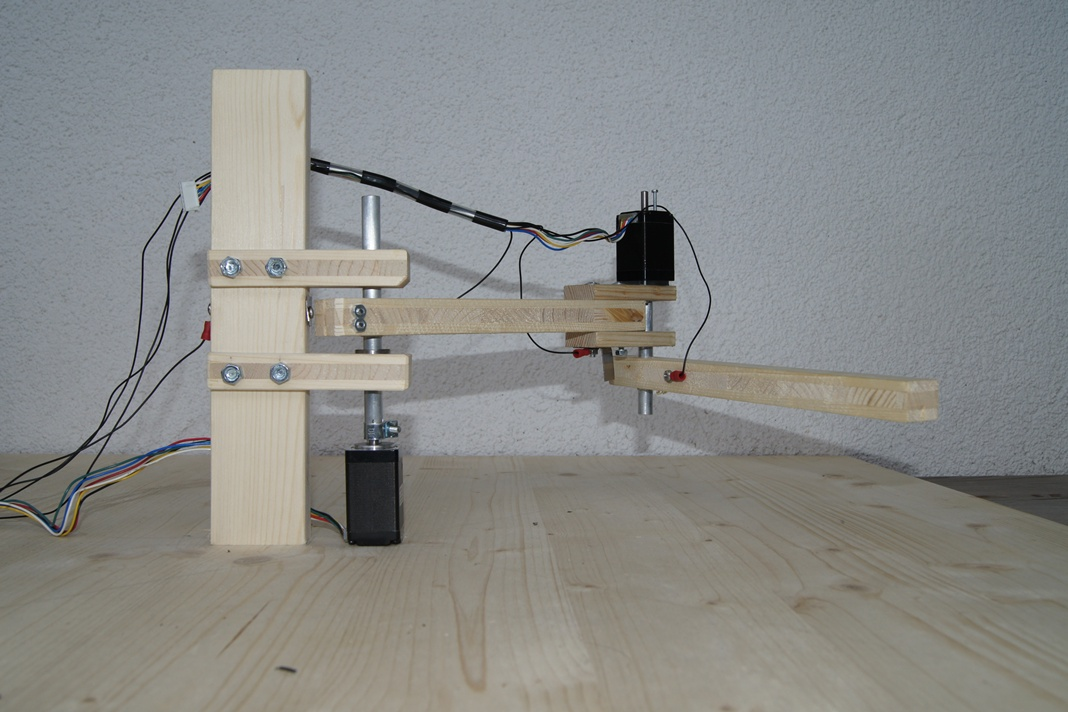
\includegraphics[width=12cm]{images/edubot_photo} 
    \caption{Das Edubot Modell}
  \end{minipage}
\end{figure}

\subsubsection{Aufgaben}
Das Edubot Modell soll als Anschauungsmaterial sowohl für den Unterricht, als für Anlässe wie den Tag der offenen Tür oder sonstige Präsentationszwecke dienen. Der Aufbau des Modells und die verwendete Elektronik wurde bewusst so simpel wie möglich gehalten um es Schülern zu ermöglichen schnell einen Überblick über die Funktionsweise und konstruktionstechnischen Eigenheiten zu erlangen.

\subsubsection{Funktionen}
Das Edubot Vorführmodell verfügt über zwei rotatorische Achsen die auf horizontaler Ebene bewegt werden können. 
Der Roboter besitzt damit zwei Freiheitsgrade und kann auf einer Ebene alle Punkte in einem Nieren-förmigen Arbeitsbereich anfahren. Abhängig vom montierten Werkzeug kann der Roboter beispielsweise dafür verwendet werden einfache Zeichnungen anzufertigen. Ein entsprechendes Werkzeug wird jedoch nicht mitgeliefert und muss selbst konstruiert werden.

\subsubsection{Bedienung}
Als Steuerungsteil des Roboterarms dient ein Mikrocontroller (GHI Embedded Master) welcher sowohl über eine Netzwerkschnittstelle, als auch über einen USB Anschluss verfügt. Zur Übergabe von Befehlen an den Roboter wird ausschließlich die Netzwerkschnittstelle verwendet. Der USB Anschluss  wird nur benötigt um Softwareänderungen am Controller durchzuführen.
Um dem Roboterarm Befehle zu übergeben, muss der Mikrocontroller mithilfe eines normalen Netzwerkkabels mit RJ-45 Steckern an einen Computer angeschlossen werden auf welchem eine Applikation läuft welche auf der mitgelieferten API aufbaut.

\subsection{Motoren}
Als Motoren wurden bei der Planung dieses Modells jene Drehstrom-Servomotoren verwendet die der Schule von der Firma Keba zur Verfügung gestellt wurden. 

Zum Betrieb der Motoren werden, ebenfalls in der Schule vorhandene, passende Motoransteuerungen benötigt. Für jeden Motor ist eine Steuerung nötig. 

Die Steuerungen werden über eine SercosII Schnittstelle mit der SPS verbunden. Die Verbindung erfolgt über normale Patch Kabel, eine Steuerung wird direkt mit der SPS verbunden, die zweite wird dann mit dieser ersten Steuerung verbunden. Über den kleinen Display an der Motorsteuerung lassen sich die benötigten Einstellungen bezüglich der Rolle die der angeschlossene Motor spielt tätigen und es muss zur einzelnen Ansteuerung jedem Motor eine Nummer gegeben werden.

\subsection{Netzwerkschnittstelle}
\subsubsection{Allgemein}
Die Netzwerkschnittstelle des KEBA Modells ist auf der SPS implementiert und soll die Kommunikation mit der Roboter API ermöglichen, diese Kommunikation verläuft über Sockets und unterscheidet sich im Prinzip wenig von jener auf dem Edubot Modell, lediglich die Art der Implementierung unterscheidet sich auf Grund der unterschiedlichen Programmierumgebungen sehr stark. Für die implentierung der Netzwerkfunktionalität wurde die frei zur Verfügung stehende OSCAT Library verwendet, welche im Kapitel "'Verwendete Technologien und Werkzeuge"' kurz erklärt wird. 

Die Netzwerkschnittstelle ist sowohl für den Empang von Befehlen und Pfaden, als auch für die Rückgabe von Statusinformationen verantwortlich und ist auf der SPS als Aufgabe ohne harte Echtzeitanforderungen definiert, da keine Hardware direkt angesteuert wird und es dadurch nicht nötig ist zu einem genau bestimmten Zeitpunkt zu arbeiten.

\subsubsection{Aufbau}
Die Netzwerkschnittstelle ist im Programm \textit{NetworkManager} implementiert und wird durch einen Entsprechenden "'Task"' in zyklischen Abständen von 200ms aufgerufen. Da nicht bei jedem Programmaufruf sämtliche Operationen wie beispielsweise die Initialisierung der für den Empfang benötigten Variablen vorgenommen werden sollen, sondern vielmehr abhängig vom aktuellen Status der Kommunikation unterschiedliche Programmteile benötigt werden, basieren zyklisch aufgerufenen Programmen meist auf einer \textit{Switch} Kontrollstruktur. Die \textit{Switch} Kontrollstruktor entscheidet mittels einer \textit{status} Variable, welche Operationen derzeit benötigt werden. In den einzelnen Fällen der \textit{Switch} Struktur befindet sich die Programmlogik die Ausgeführt werden soll wenn die \textit{status} Variable den Wert dieses Falles annimmt. Üblicherweise ist der ist der Anfangswert der \textit{status} Variable 0, wodurch beim ersten zyklischen Aufruf des Programms die dem Fall 0 zugeordnete Programmlogik ausgeführt wird. Diese Programmlogik kann beispielsweise zur Initialisierung von Variablen dienen. Wurde die Inititialisiierung, um kurz an diesem Beispiel festzuhalten, erfolgreich beendet, so wird im Fall 0 noch die \textit{status} Variable so gesetzt, dass beim nächsten Programmaufruf die nach der initialisierung auszuführende Programmlogik ausgeführt wird. Dieses Prinzip kann nun innerhalb des Programms beliebig fortgeführt werden.

\subsubsection{Umsetzung}
Auf die genau Implementierung der Netzwerkkommunikation auf der SPS wird hier nur oberflächlich eingegangen, genauere Informationen hierzu sind der Dokumentation der OSCAT Network Library und dem Source Code der SPS zu entnehmen, welcher im Rahmen der Diplomarbeit gemeinsam mit der restlichen Software des Edubot Systems abgegeben wurde. Im Folgenden erfolgt lediglich eine Kurze Aufzählung der wichtigsten Objekte und ihrer Verwendung:
\begin{itemize}
\item \textbf{IP\_CONTROL}\\
Der Typ IP\_CONTROL ist der zentrale Baustein einer Netzwerkkommunikation mit OSCAT. Über ein Objekt dieses Typs werden alle wichtigen Operationen zur Komunikation, wie beispielsweise das anlegen eines Sockets und das Empfangen der Daten abgewickelt. Zum Verbindungsaufbau über ein IP\_CONTROL Objekt ist es lediglich Nötig, dieses mit den entsprechenden Parametern anzulegen und in periodischen Abständen zu Überprüfen ob bereits eine Verbindung hergestellt wurde, dies geschieht über das state Attribut des IP\_CONTROL Objekts, welches jederzeit den Verbindungsstatus in Form eines Integer Wertes beinhaltet, die möglichen Werte dieses Attributs sind der OSCAT Network Library Dokumentation zu entnehmen

\item \textbf{IP\_C}\\
Zur Erzeugung eines IP\_CONTROL Objekts muss ein IP\_C Objekt übergeben werden, welches alle nötigen Parameter für die Verbindung enthält. Zwar verfügt das IP\_CONTROL selbst bereits über einige entsprechende Attribute, diese sollten jedoch nur als default Werte verwendet und von denen im IP\_C Objekt überschrieben werden. 
Wichtige Attribute eines IP\_C Objekts sind zum Beispiel C\_MODE, welches angibt welche Art der Verbindung aufgebaut werden soll, C\_ENABLE zum freigeben der Verbindung und R\_OBSERVE zur Aktivierung des Dateiempfangs.

\item \textbf{NETWORK\_BUFFER}\\
Bei der Erzeugung eines IP\_CONTROL Objekts muss um das Senden beziehungsweise Empfangen von Nachrichten zu ermöglichen je ein Objekt vom Typ NETWORK\_BUFFER als Lesebuffer und eines als Schreibbuffer mitgegeben werden. Ein Objekt vom Typ NETWORK\_BUFFER ist grundsätzlich dazu da entweder empfangene Daten zu einem Stream zu Sammeln um sie später komfortabel auslesen zu können oder zu sendende Daten für die Netzwerkübertragung aufzubereiten um sie später als den zulässigen Blockgrößen entsprechende Pakete zu versenden.
\end{itemize}

\subsubsection{Ablauf des Datenempfanngs}

Um eine Netzwerkverbindung herzustellen muss zuerst ein IP\_C Objekt zur Speicherung der Verbindungsparameter (siehe Kapitel "'Umsetzung"') angelegt werden.
Ebenfalls vor Beginn der Kommunikation müssen zwei NETWORK\_BUFFER Objekte für das Senden und Empfangen von Daten angelegt und initialisiert werden. 
Wie bereits im Kapitel "'Aufbau"' beschrieben, basiert die Netzwerkkomunikation auf einem zyklisch aufgerufenen Programm, welches über einen \textit{Integer} Variable die aktuell auszuführende Operation definiert. Die eben beschriebenen Operationen sollen am Anfang des Programms und somit wenn die \textit {state} Variable auf ihren Initialwert 0 gesetzt ist ausgeführt werden. Nach der Ausführung dieser Schritte wird \textit {state} so gesetzt dass beim nächsten Programmaufruf der nächste Schritt ausgführt wird, in unserem Fall wird \textit{state} auf 10 gesetzt.

Als nächster Schritt (\textit{state} = 10) muss nun ein  IP\_CONTROL aufgerufen werden. Die vorher instanzierten Objekte hierbei werden direkt übergeben. Durch diesen Schritt beginnt die SPS auf eingehende Verbindungen zu horchen.
Ein Beispiel für den Aufruf des IP\_CONTROL's sieht folgendermaßen aus:

IP\_CONTROL1(PORT:=400 ,TIME\_OUT:=T\#1s,IP\_C:= IP\_C1,S\_BUF:=S\_BUF1, R\_BUF:=R\_BUF1 );

Durch regelmäßiges überprüfen des \textit{state} Attributs des IP\_CONTROL Objektes kann nun festgestellt werden wenn eine neue Verbindung hergestellt wurde. Bekommt das \textit{state} Attribut des IP\_CONTROLs den Wert 254, so wurde die Verbindung erfolgreich aufgebaut und es kann zum Datenempfang übergegangen werden. Hierzu wird die \textit{state} Variable des Programms auf 30 gesetzt.

Während des Wartens auf Dateiempfang (\textit{state} = 30) wird in regelmäßigen Abständen das \textit{size} Attribut des dem IP\_CONTROLL mitgegebenen NETWORK\_BUFFER Objekts - im obigen Beispielfall R\_BUF1 - überprüft. Nimmt das \textit{size} Attribut einen Wert an der höher als 0 ist, so wurden Daten empfangen und können aus dem NETWORK\_BUFFER ausgelesen werden. Der NETWORK\_BUFFER enthält hierzu ein array aus \textit{byte} Werten welches werden kann. Die einzelnen Byte Werte werden mithilfe einer einfachen selbst geschriebenen Funktion (siehe BYTE\_TO\_CHAR Funktion im Kapitel "'Hilfsfunktionen"') in eine Zeichenkette umgewandelt. Die \textit{state} Variable wird dannach auf den Wert 40 gesetzt um im nächsten Programmdurchlauf die empfangene Zeichenkette zu analysieren.

Liegt die übertragene Nachricht als Zeichenkette vom Typ \textit{string} vor (\textit{state = 40}), so werden zuerst ihre ersten drei Buchstaben überprüft. Diese drei Buchchstaben enthalten, ähnlich wie beim Edubot Modell, die Information welche Operation ausgeführt werden soll. 
Abhängig von der zu tätigenden Operation werden nun globale Variablen verändert, Daten konvertiert. Die folgende Auflistung gibt an welche Aktionen bei Empfang der wichtigsten Befehle ausgeführt werden:

\begin{itemize}
\item \textbf{Befehl "mvs"}\\
Der Befehl informiert die Steuerung darüber, dass eine lineare Bewegung ausgeführt werden soll. Enthält die Empfangene Zeichenkette diesen Befehl in ihren ersten drei Zeichen, so enthält der rest der Zeichenkette alle zum Abfahren dieser Bewegung benötigten Punkte.
Mit Hilfe einer weiteren selbst geschriebenen Funktion (siehe "'InterpretToGlobalStepArray"' Funktion im nächsten Kapitel "'Hilfsfunktionen"') wirden die in der Zeicehnkette enthaltenen Interpolationspunkte in Arrays vom Typ Real (Gleitkommadatentyp) umgewandelt und als globale Variablen abgelegt. Hierbei wird für jede Achse ein Array angelegt das für jeden Intapolationsschritt den richtigen Winkel angiebt. Aus diesem Array liest später der für die Bewegung zuständige "'MotionTask"' die aktuell zu verfahrenden Winkel aus und übergiebt sie an die Motorsteuerung um die Bewegung phsysisch durchzuführen. Dieser Vorgang ist im Unterkapitel "'Steuerung der Motoren"'' genauer erklärt. Zusätz
\item \textbf{Befehl "hom"}\\
Enthält die empfangene Zeichenkette als Präfix die Zeichen "hom", so wird der Steuerung bekannt gegeben dass der Roboter seine Ausgangsposition suchen soll. Da zum aktuellen Zeitpunkt keine Hardware zur Verfügung stand konnte dieser Vorgang nicht implementiert werden und es wird hier lediglich ein globaler \textit{boolean} Wert auf \textit{true} gesetzt welche später "'MotionTask"' den "'Homing Prozess" auslösen soll.'
\item \textbf{Befehl "sht"}\\
Der Befehl "sht" dient dazu den Roboter auszuschalten, also alle Motoren zu deaktivieren und sonstige zum herunterfahren nötige Abläufe durchzuführen. 
\end{itemize}

\subsubsection{Hilfsfunktionen}
Um diverse Umrechnungen zu vereinfachen und redundaten Programmcode zu vermeiden wurden diverse Hilfsunktionen erzeugt die an enprechnder Stelle im\textit{ NetworkManager} Programm verwendet werden, die folgende Auflistung soll einen Überblick über diese Funktionen bieten, Informationen über ihre Funktionalität bereitstellen und ihre Verwendung im Programm kurz beschreiben:

\begin{itemize}
\item \textbf{BYTE\_TO\_CHAR}\\
Da von CoDeSys standardmäßig keine Funktion zur umrechnung eines \textit{byte} Wertes in einen \textit{char} Wert zur Verfügung gestellt wird, diese aber für die Umrechnung des empfangenen \textit{byte} Arrays in einen String benötigt wird, musste eine entsprechende Funktion selbst erzeugt werden. Die beschriebene Funktion erhält als input Parameter einen einzelnen \textit{byte} Wert und gibt einen Einstelligen \textit{string} Wert zurück, welcher als Inhalt den umgerrechneten \textit{byte} Wert enthält. Das \textit{NetwokManager} Programm ruft diese Funktion innerhalb einer Schleife auf welcher das empfangene \textit{byte} Array mit Hilfe einer Schleife durchläuft und die Ergebnisse der Umrechnung zu einem einzigen String zusammenfügt.

\item \textbf{CHAR\_TO\_BYTE}\\
Diese Funktion bildet das Gegenstückk zur im letzten Schritt beschriebenen Methode, sie wandelt einzelne \textit{char} Werte in Bytes um. Dies ist notwendig um im \textit{NetwokManager} Programm den an den Computer zu sendenden, als \textit{string} vorliegeneden Status  in ein sendbares \textit{byte} Array umzuwandeln, auch hier kommt wieder eine Schleife zur einzelnen Umwandlung aller im \textit{string} enthaltenen Zeichen zum Einsatz.

\item \textbf{InterpretToGlobalStepArray}\\
Da die Empfangenen Schrittinformation in Form einer Zeichenkette nicht direkt vom "'Motion Task" verwendet werden kann, ist es notwendig diese vorher in einzelne Arrays für jeden Motor zu zerlegen. Hierzu wird der Funktion \textit{InterpretToGlobalStepArray} die zu konvertierende Zeichenkette übergeben. In der Funktion selbst wird die Zeichenkette wiederum in einzelne Zeichenketten zerlegt die jeweils die zu verfahrenden Winkel für einen einzelnen Schritt pro Motor angeben. Diese Zeichenkette wird zur Umwandlung der Winkelstellungen in Werte vom Typ \textit{real} der Hilfsfunktion \textit{InterpretToAngles} überbeben. Das von der genannten Funktion zurückgegebene Array enthält nun gewünschten Winkel in Werten vom Typ \textit{real}. Diese Werte werden nun in die globalen Array der einzelnen Motoren angefügt. Nach Umwandlung aller Werte wird schließlich die globale Variable \textit{stepsAvailable} auf die Anzahl der konvertierten Schritte gesetzt. Zusätzlich wird die globale Variable \textit{robot\_ready} auf \textit{false} gesetzt.

\item \textbf{InterpretToAngles}\\
Diese Funktion dienst dazu, die in Form einer Zeichenkette als Parameter übergebenen Winkel eines einzelnen Interpolationsschrittes in ein Array vom Typ \textit{real} umzuwandeln und zurückzugeben.

\end{itemize}

\subsubsection{Der Rückmelde-Prozess}
Wurden der Datenempfang und alle im \textit{NetworkManager} durchzuführenden Operation zur ordnungsgemäßen Abarbeitung der Befehle abgeschlossen, so wird wie im Kapitel "'Ablauf des Dateiempfang"' bereits erwähnt, die \textit{state} Variable des Programms auf 110 gesetzt. Befindet sich das Programm in diesem Zustand, so werden bei jedem Aufruf globale Statusvariablen überprüft um bei bestimmten Veränderungen eine entsprechende Rückmmeldung an den Verbundenen Computer zu geben. Die wichtigsten Variablen sind hierbei \textit{robot\_ready}, \textit{robot\_shutdown} und \textit{robot\_failure}.

Ist die \textit{robot\_ready} Variable auf \textit{true} gesetzt, so sendet das \textit{NetworkManager} wird zuerst eine Zeichenkette mit dem Wert "'ready"' erzeugt, mithilfe einer Schleife und der der Hilfsfunktion CHAR\_TO\_BYTE in einzelne Bytes zerlegt und dem zum Senden vorgesehenen NETWORK\_BUFFER Objekt übergeben. In unserem Fall trägt dieses Objekt den Namen "'S\_BUFF1"'. Nun kann durch Aufruf des IP\_CONTROLLs die Zeichenkette an den Computer übergeben werden um zu signalisieren dass der Roboter bereit ist neue Befehle zum empfangen. Nach Beendigung der Übertragung wird die \textit{state} Variable des Programms auf den Wert 30 gesetzt um beim nächsten Aufruf wieder auf Daten zu horchen.

Befinden sich hingegen entweder die globale Variable \textit{robot\_shutdown} oder \textit{robot\_failure} im Status \textit{true}, so wird die Zeichenkette "'shutdown"' in konvertiert und dem Sendebuffer übergeben. Damit wird dem Computer mitgeteilt dass der Roboter derzeit nicht verwendbar ist und entweder heruntergefahren wurde oder ein Fehler aufgetreten ist. In beiden Fällen muss eine neue Verbindung mit der Steuerung hergestellt werden und somit der "'Homing Prozess"' durchgeführt werden. Nach dem Senden dieser Mitteilung wird die Verbindung beendet und die \textit{state} Variable wird auf 0 gesetzt um das \textit{NetworkManager} Programm neu zu initialisieren. 

Um die Verbindung zu beenden muss Aufgrund eines Fehler in der OSCAT Library zuerst der Socket manuell geschlossen werden, dies passiert am Beispiel der Steuerungssoftware mit folgender Zeile:

SysSockClose(diSocket:=IP\_CONTROL1.socket);

Wurde dieser Schritt ausgeführt kann über das C\_ENABLED Attribut des übergebenen IP\_C Objekts das IP\_CONTROL abgeschaltet werden.




\subsection{Motoransteuerung}
Diese Kapitel behandelt Programmvorgänge die in der SPS nötig sind, um die Motoren mit eine korrekte Bahn fahren zu lassen. Welche Voraussetzungen aus Sicht der Hardware gegeben sein müssen ist dem Kapitel "'Motoren"' zu entnehmen.

\subsubsection{Vorgehensweise}
Anfangs war geplant für die Steuerung der Motoren die internen Interpolationsfunktionen der KEBA Steuerung zu verwenden, welche im Rahmen des Zusatzsystems KeMotion zur Verfügung gestellt werden. KeMotion ist eine Softwarekomponente die für KEBA Steuerungen angeboten wird und umfangreiche Funktionen zum Betrieb von Industrierobotern zur Verfügung stellt.
Leider ist das KeMotion System dafür ausgelegt Pfadinformationen in Form von Vorgefertigten Dateien des Dateityps KAIRO zu Verarbeiten. Es ist vorgesehen dass diese Dateien, welche die anzufahrenden Punkte in Form einer einfachen Scriptsprache (ähnlich einer CNC Programmiersprache) enthalten, bereits beim Programmstart vorhanden sind oder mithilfe eines geeigneten Teach-In Geräts (Gerät zur Eingabe der Bahn) erzeugt werden. Diese Eigenheit bereitete unverhältnismäßig große Schwierigkeiten da im Edubot-System die Punkte über die Netzwerkschnittstelle übergeben werden und so erst zur Laufzeit auf das Gerät gelangen. 
Aus diesem Grund und basierend auf der Tatsache dass die Edubot API ebenfalls über funktionstüchtige Mechanismen für Bahninterpolation und Invers-Kinematik verfügt, fiel der Entschluss, ähnlich wie beim Edubot Modell bereits fertig interpolierte Bahnen in Form einer Liste an Punkten zu übergeben. Ein Vorteil dieser Vorgehensweise ist die bessere Überschaubarkeit der Steuerungssoftware, wodurch die Möglichkeit gegeben ist sie optimal für Schulungszwecke einzusetzen.

\subsubsection{Basiseinstellungen}
Um die Ansteuerung der Motoren grundsätzlich zu ermöglichen, ist es nötig im Menüpunkt "'PLC Configuration"' in KeStudio einen neuen Knotenpunkt anzulegen. Dieser Knotenpunkt ist vom Typ "'Drives SercosIII"' und dient als übergeordnetes Element für alle über die SercosIII Schnittstelle angeschlossenen Motoren. 
Es können nun neue Unterelemente für den angelegten Knotenpunkt erzeugt werden. Diese Unterpunkte haben den Typ "'Drive SercosIII"' und repräsentieren jeweils einen einzelnen Motor. Es muss nun noch jedem Motor ein entsprechender Name gegeben werden über den er später aus dem Programmcode ansprechbar sein soll. Zusätzlich muss für die einzelnen Motoren jeweils die "'Node-ID"' angegeben werden, also jene Nummer die auf der Steuerung des Motors unter dem Menüpunkt "'Slave"' festgelegt wurde.

\begin{figure}[H]
  \centering
  \begin{minipage}[t]{9 cm}
  	\centering
  	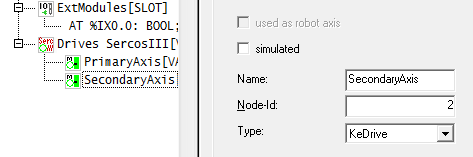
\includegraphics[width=9 cm]{images/DriveConfiguration} 
    \caption{Basiskonfiguration des sekundären Motors}
  \end{minipage}
\end{figure}

\subsubsection{Der Motion Task}
Der "'Motion Task"' dient dazu die Winkelstellungen der Motoren zu aktualisieren, hierzu wird in vom System vorgegebenen Abständen das Programm \textit{McMain} aufgerufen. Das genannte Hauptprogramm überprüft zuerst ob alle zur initialisierung notwendigen Schritte getätigt wurden und geht dann dazu über zuerst die aktuellen Winkelstellungen auszulesen, neue Soll-Werte zu setzen und diese Schließlich an die Motorsteuerungen weiterzugeben. 

Das setzen der neuen Winkelstellungen, sowie alle anderen Operation die eine Veränderung des Zustands der Motoren mit sich bringen passiert im Programm \textit{UserUpdate} welches zwischen dem Lesen der Ist-Werte und dem schreiben der Soll-Werte aufgerufen wird.

\subsubsection{Das UserUpdate Programm}
Das \textit{UserUpdate} Programm dient wie bereits erwähnt zum verändern des Zustands der Motoren. Das Programm ähnelt im Aufbau dem \textit{NetworkManager} Programm sehr stark da es ebenfalls über eine \textit{Switch} Kontrollstruktur gesteuert wird. Für eine genauere Beschreibung dieser Art von Programmaufbau siehe Unterkapitel "'Aufbau"' im Kapitel "'Die Netzwerkkommunikation"'.

Im initialen Status (\textit{state} = 0) beginnt das \textit{UserUpdate} Programm zuerst damit die einzelnen Motoren zu "'resetten"', dies ist notwendig um etwaige Fehler oder unbrauchbare Einstellungen aus der Motorsteuerung zu löschen. Die Operationen an den Motoren werden jeweils über vom System bereitgestellte Funktionsblöcke durchgeführt, welche zur richtigen Zeit mit den entsprechenden Parametern aufgerufen werden. Meist verfügt ein für eine Operation nötiger Funktionsblock über einen \textit{Execute} Parameter, welcher eine positive Flanke aufweisen muss damit die Operation durchgeführt wird. Aus diesem Grund ist es nötig die Funktionsblöcke zweimal aufzurufen, am Beispiel der "'reset"' Operation sieht dies folgendermaßen aus:
\begin{lstlisting}[language = codesysls, captionpos=b, caption={Resetten einer Motors}]
fb_reset_primaryAxis(Axis := SecondaryAxis, Execute := FALSE);
fb_reset_primaryAxis(Axis := SecondaryAxis, Execute := TRUE);
\end{lstlisting}

Nachdem dieser Schritt ausgeführt wurde, wird \textit{state} auf 1 gesetzt. 

Befindet sich das Programm im Status 1, so wird zuerst überprüft ob das "'resetten"' der Motorsteuerungen abgeschlossen ist. Ist dies der Fall, so wird der Funktionsblock für das "'resetten"' erneut aufgerufen um dem \textit{Execute} Parameter den Wert \textit{FALSE} zuzuweisen und damit den Motor für weitere Operationen freizugeben.
Nach Abschluss dieser Operation wird die \textit{state} Variable des Programms auf 10 gesetzt um beim nächsten Programmaufruf die Motoren einzuschalten.

Der nächste Schritt im Programm ist das Einschalten der Motoren, dies geschieht wieder über Aufruf des entsprechenden Funktionsblocks (\textit{MC\_Power}, muss zuvor instanziert worden sein). War das Einschalten der Motoren erfolgreich, so wechselt das Programm in den Status 12.

Im Status 12 überprüft das \textit{UserUpdate} Programm ob ein "'Homing"' also eine Suche nach der Ausgangsposition durchgeführt werden muss. Diese Überprüfung findet mithilfe der globalen Variable \textit{robot\_homing} stattd die gegebenenfalls durch das \textit{NetworkManager} Programm auf den Wert \textit{true} gesetzt wurde.
Da im Rahmen dieses Projektes keine Mechanik erstellt wurde, war das eigentliche "'Homing"' nicht implementierbar und es wird hier Fall lediglich die globale Variable \textit{robot\_homing} auf \textit{false} gesetzt. Zusätzlich wird die globale Variable \textit{robot\_ready} auf \textit{true} gesetzt um dem \textit{NetworkManager} Programm zu signalisieren dass der Roboter bereit ist Befehle zu empfangen. Das \textit{NetworkManager} Programm gibt diese Information an den Computer weiter. Am Ende wird die \textit{state} Variable auf 20 gesetzt.

Hat die \textit{state} Variable den Wert 20, so wartet der "'Motion Task"' auf neue Interpolationspunkte in Form von Winkelstellungen. Werden neue Interpolationspunkte durch das \textit{NetworkManager} Programm eingelesen, so werden sie in globale Array gespeichert, siehe Unterkapitel "'Ablauf des Datenempfanngs"' im Kapitel "'Netzwerkkommunikation"'. Wenn alle Werte fertig eingelesen wurden, wird die globale Variable \textit{stepsAvailable} auf die Länge des Array gesetzt. Hat die genannte Variable nun einen Wert der höher als 0 ist, so wird der erste Winkel aus dem Array an die Motorsteuerung als relativ zu verfahrender Winkel weitergegeben. Die Variable \textit{stepsAvailable} wird nun um 1 verringert und die Variable \textit{curStepIndex} wird um 1 erhöht. Die genannte \textit{curStepIndex} Variable ist zu Anfang 0 und dient dazu zu speichern welcher Schritt aus dem Array beim nächsten Aufruf des \textit{UserUpdate} Programms gefahren werden soll.
\begin{lstlisting}[language = codesysls, captionpos=b, caption={Übergabe der Winkel an die Motoren}]
20: (* Start relative Movement *)

		IF(stepsAvailable > 0)THEN

		fb_moveRelative_primaryAxis(Axis := PrimaryAxis, Execute := FALSE);
		fb_moveRelative_primaryAxis(Axis := PrimaryAxis, Execute := TRUE, Distance := primarySteps[currentStepIndex], Velocity := 300, Acceleration := 10000, Deceleration := 10000);

		fb_moveRelative_secondaryAxis(Axis := SecondaryAxis, Execute := FALSE);
		fb_moveRelative_secondaryAxis(Axis := SecondaryAxis, Execute := TRUE, Distance := primarySteps[currentStepIndex], Velocity := 300, Acceleration := 10000, Deceleration := 10000);

		currentStepIndex := currentStepIndex +1;
		stepsAvailable := stepsAvailable -1;
		END_IF;
\end{lstlisting}

Wurden alle Schritte gefahren, so wird die Variable \textit{robot\_ready} auf true gesetzt. 

Wird im Status 20 durch Kontrolle der \textit{robot\_shutdown} Variable erkannt dass der Roboter heruntergefahren werden soll, so wird \textit{state} auf 100 gesetzt. Damit werden beim nächsten Aufruf des Programms die  Motoren abgeschaltet.






\subsection{Konstruktion des Modells}
\subsubsection{Allgemein}
Im Rahmen dieses Projektes wurden bereits umfangreiche Überlegungen angestellt, wie ein stabileres, leistungsstärkeres Modell unter Verwendung der größeren Motoren der Firma KEBA verwirklicht werden könnte.
Grundsätzlich basierten alle Überlegungen bezüglich der Konstruktion dieses Modells auf einer Fertigung aus Aluminium. Hierfür wurden im Projektverlauf die entsprechenden Aluminiumprofile beschafft, welche später beim Bau noch auf die optimale Länge zurecht geschnitten werden müssen. 
Im Zuge dieser Überlegungen wurde auch ein Aluminiumrohling in Form einer 16 mm Dicken Platte beschafft aus dem die Teile des Gelenks gefräst werden sollen.

\subsubsection{Gelenke}
Einen Knackpunkt bei der Konstruktion des Aluminiummodells stellte der Aufbau der einzelnen Gelenke dar. Die schlussendlich gewählte Herangehensweise wurde bereits in dieser Diplomarbeit im Kapitel "'Komponenten des Edubot Modells"' beschrieben. Grundgedanke der Gelenke ist die Erzeugung eines Bauteils der grob gesagt aussieht wie ein liegendes U. In den beiden Längsseiten des Us befinden sich Kugellager durch welche eine Verlängerung der Motorwelle führt. 
An diese Wellenverlängerung wird dann der eigentliche Arm befestigt. Durch diese Konstruktionsweise werden alle Kräfte die durch das Gewicht des Armes entstehen durch die Kugellager getragen und haben keinen Einfluss auf die Laufeigenschaften des Motors.

\subsection{CNC Programmierung}
Die einzelnen Bauteile die zum Bau der im vorherigen Unterkapitel beschriebenen U-Förmigen Gelenke nötig sind wurden im Rahmen dieses Projektes als CNC Programm geschrieben und liegen dieser Arbeit bei. Als Werkzeug für die Erstellung der CNC Programme wurde die Software WinNC der Firma EMCO verwendet, welche in weiterer Folge auch für die Ausführung der Programme auf der schuleigenen Fräse verwendet werden kann. 
Grundsätzlich sind beim schreiben eines CNC Programmes nur die durch die Fräse auszuführenden Bewegungen und die jeweils benötigten Werkzeugoperationen aufzulisten. Für spezielle Operationen, wie beispielsweise das Fräsen einer Tasche oder das Bohren eines Gewindes stehen bereits vorgefertigte Operationen zur Verfügung die mit den richtigen Parametern aufgerufen werden müssen.
Leider gab es bei der Verwendung der WinNC Software Probleme mit der Lizenz, so dass zum Zeitpunkt der Anfertigung dieser schriftlichen Arbeit eine Simulation der CNC Programme nicht möglich war. Aus diesem Grund können hier keine Abbildungen gezeigt werden um die Einzelnen Bauteile zu präsentieren. Die Folgende Abbildung zeigt jedoch den einen Ausschnitt aus dem CNC Programm dass zur Erstellung eines Seitenteils des Gelenks verwendet werden kann, der gezeigte Ausschnitt dient dazu, Taschen für die Kugellager zu fräsen.

\begin{figure}[H]
\centering
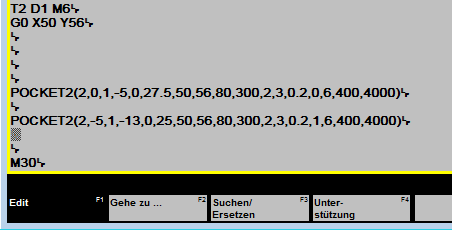
\includegraphics[width=9cm]{images/cncprogramm}
\caption{Screenshot eines CNC Programms in WinNC}
\end{figure}

\subsection{Sonstige Überlegungen}
Während der Planung der Mechanik des größeren Modells kamen wir unter Anderem zu dem Schluss, dass die Motoren nicht direkt mit den Armen verbunden werden sollten, sondern dass hier als Zwischenglied eine Übersetzung von Vorteil wäre. Diese Feststellung resultiert vor allem aus der Tatsache, dass die verwendeten Motoren sehr hohe Drehzahlen erreichen können und ihr maximaler Drehmoment im Gegenzug sehr begrenzt ist.


	\newpage
	
\label{chap:keba}

\section{Komponenten des KEBA Modells}


\subsection{Allgemein}            
Der Name Edubot bezeichnet sowohl das Softwaresystem als ganzes, als auch den aus Holz gefertigten Roboterarm. Der Roboterarm wird um Missverständnisse zu vermeiden allgemein als "'Edubot Modell"' bezeichnet. Es handelt sich bei diesem Roboterarm um eine Konstruktion mit zwei rotatorischen Achsen die so konzipiert wurde dass eine Erweiterung um diverse Werkzeuge oder weitere Achsen ohne Probleme und mit Hilfe des Handbuchs möglich ist. 

\begin{figure}[H]
  \centering
  \begin{minipage}[t]{12 cm}
  	\centering
  	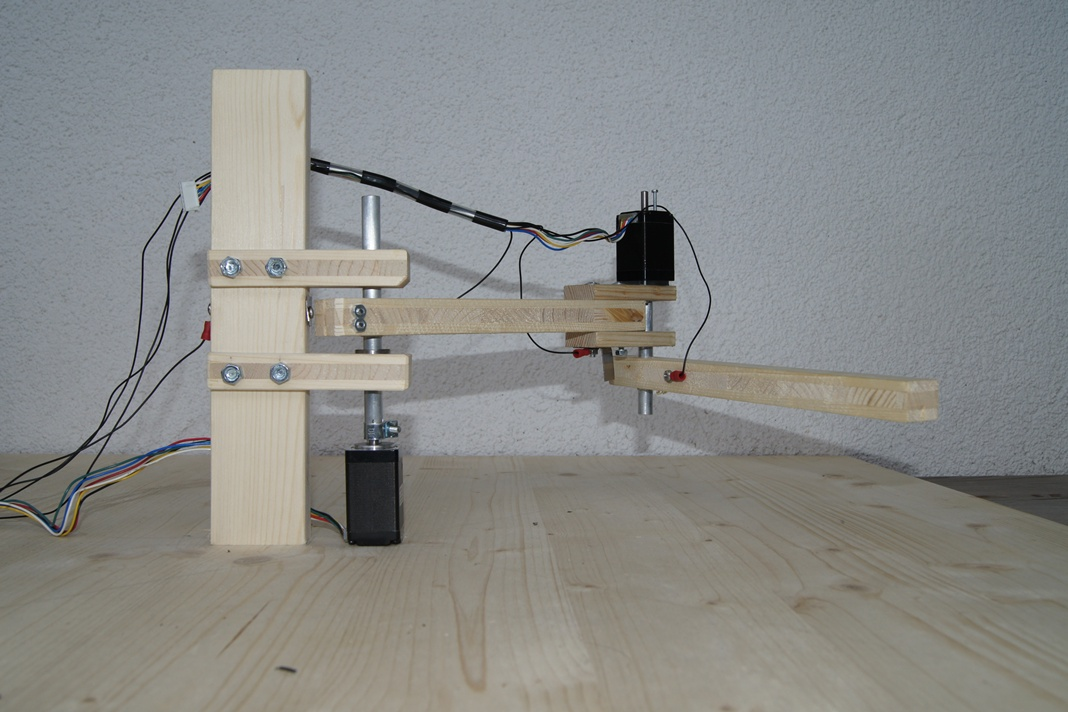
\includegraphics[width=12cm]{images/edubot_photo} 
    \caption{Das Edubot Modell}
  \end{minipage}
\end{figure}

\subsubsection{Aufgaben}
Das Edubot Modell soll als Anschauungsmaterial sowohl für den Unterricht, als für Anlässe wie den Tag der offenen Tür oder sonstige Präsentationszwecke dienen. Der Aufbau des Modells und die verwendete Elektronik wurde bewusst so simpel wie möglich gehalten um es Schülern zu ermöglichen schnell einen Überblick über die Funktionsweise und konstruktionstechnischen Eigenheiten zu erlangen.

\subsubsection{Funktionen}
Das Edubot Vorführmodell verfügt über zwei rotatorische Achsen die auf horizontaler Ebene bewegt werden können. 
Der Roboter besitzt damit zwei Freiheitsgrade und kann auf einer Ebene alle Punkte in einem Nieren-förmigen Arbeitsbereich anfahren. Abhängig vom montierten Werkzeug kann der Roboter beispielsweise dafür verwendet werden einfache Zeichnungen anzufertigen. Ein entsprechendes Werkzeug wird jedoch nicht mitgeliefert und muss selbst konstruiert werden.

\subsubsection{Bedienung}
Als Steuerungsteil des Roboterarms dient ein Mikrocontroller (GHI Embedded Master) welcher sowohl über eine Netzwerkschnittstelle, als auch über einen USB Anschluss verfügt. Zur Übergabe von Befehlen an den Roboter wird ausschließlich die Netzwerkschnittstelle verwendet. Der USB Anschluss  wird nur benötigt um Softwareänderungen am Controller durchzuführen.
Um dem Roboterarm Befehle zu übergeben, muss der Mikrocontroller mithilfe eines normalen Netzwerkkabels mit RJ-45 Steckern an einen Computer angeschlossen werden auf welchem eine Applikation läuft welche auf der mitgelieferten API aufbaut.

\subsection{Motoren}
Als Motoren wurden bei der Planung dieses Modells jene Drehstrom-Servomotoren verwendet die der Schule von der Firma Keba zur Verfügung gestellt wurden. 

Zum Betrieb der Motoren werden, ebenfalls in der Schule vorhandene, passende Motoransteuerungen benötigt. Für jeden Motor ist eine Steuerung nötig. 

Die Steuerungen werden über eine SercosII Schnittstelle mit der SPS verbunden. Die Verbindung erfolgt über normale Patch Kabel, eine Steuerung wird direkt mit der SPS verbunden, die zweite wird dann mit dieser ersten Steuerung verbunden. Über den kleinen Display an der Motorsteuerung lassen sich die benötigten Einstellungen bezüglich der Rolle die der angeschlossene Motor spielt tätigen und es muss zur einzelnen Ansteuerung jedem Motor eine Nummer gegeben werden.

\subsection{Netzwerkschnittstelle}
\subsubsection{Allgemein}
Die Netzwerkschnittstelle des KEBA Modells ist auf der SPS implementiert und soll die Kommunikation mit der Roboter API ermöglichen, diese Kommunikation verläuft über Sockets und unterscheidet sich im Prinzip wenig von jener auf dem Edubot Modell, lediglich die Art der Implementierung unterscheidet sich auf Grund der unterschiedlichen Programmierumgebungen sehr stark. Für die implentierung der Netzwerkfunktionalität wurde die frei zur Verfügung stehende OSCAT Library verwendet, welche im Kapitel "'Verwendete Technologien und Werkzeuge"' kurz erklärt wird. 

Die Netzwerkschnittstelle ist sowohl für den Empang von Befehlen und Pfaden, als auch für die Rückgabe von Statusinformationen verantwortlich und ist auf der SPS als Aufgabe ohne harte Echtzeitanforderungen definiert, da keine Hardware direkt angesteuert wird und es dadurch nicht nötig ist zu einem genau bestimmten Zeitpunkt zu arbeiten.

\subsubsection{Aufbau}
Die Netzwerkschnittstelle ist im Programm \textit{NetworkManager} implementiert und wird durch einen Entsprechenden "'Task"' in zyklischen Abständen von 200ms aufgerufen. Da nicht bei jedem Programmaufruf sämtliche Operationen wie beispielsweise die Initialisierung der für den Empfang benötigten Variablen vorgenommen werden sollen, sondern vielmehr abhängig vom aktuellen Status der Kommunikation unterschiedliche Programmteile benötigt werden, basieren zyklisch aufgerufenen Programmen meist auf einer \textit{Switch} Kontrollstruktur. Die \textit{Switch} Kontrollstruktor entscheidet mittels einer \textit{status} Variable, welche Operationen derzeit benötigt werden. In den einzelnen Fällen der \textit{Switch} Struktur befindet sich die Programmlogik die Ausgeführt werden soll wenn die \textit{status} Variable den Wert dieses Falles annimmt. Üblicherweise ist der ist der Anfangswert der \textit{status} Variable 0, wodurch beim ersten zyklischen Aufruf des Programms die dem Fall 0 zugeordnete Programmlogik ausgeführt wird. Diese Programmlogik kann beispielsweise zur Initialisierung von Variablen dienen. Wurde die Inititialisiierung, um kurz an diesem Beispiel festzuhalten, erfolgreich beendet, so wird im Fall 0 noch die \textit{status} Variable so gesetzt, dass beim nächsten Programmaufruf die nach der initialisierung auszuführende Programmlogik ausgeführt wird. Dieses Prinzip kann nun innerhalb des Programms beliebig fortgeführt werden.

\subsubsection{Umsetzung}
Auf die genau Implementierung der Netzwerkkommunikation auf der SPS wird hier nur oberflächlich eingegangen, genauere Informationen hierzu sind der Dokumentation der OSCAT Network Library und dem Source Code der SPS zu entnehmen, welcher im Rahmen der Diplomarbeit gemeinsam mit der restlichen Software des Edubot Systems abgegeben wurde. Im Folgenden erfolgt lediglich eine Kurze Aufzählung der wichtigsten Objekte und ihrer Verwendung:
\begin{itemize}
\item \textbf{IP\_CONTROL}\\
Der Typ IP\_CONTROL ist der zentrale Baustein einer Netzwerkkommunikation mit OSCAT. Über ein Objekt dieses Typs werden alle wichtigen Operationen zur Komunikation, wie beispielsweise das anlegen eines Sockets und das Empfangen der Daten abgewickelt. Zum Verbindungsaufbau über ein IP\_CONTROL Objekt ist es lediglich Nötig, dieses mit den entsprechenden Parametern anzulegen und in periodischen Abständen zu Überprüfen ob bereits eine Verbindung hergestellt wurde, dies geschieht über das state Attribut des IP\_CONTROL Objekts, welches jederzeit den Verbindungsstatus in Form eines Integer Wertes beinhaltet, die möglichen Werte dieses Attributs sind der OSCAT Network Library Dokumentation zu entnehmen

\item \textbf{IP\_C}\\
Zur Erzeugung eines IP\_CONTROL Objekts muss ein IP\_C Objekt übergeben werden, welches alle nötigen Parameter für die Verbindung enthält. Zwar verfügt das IP\_CONTROL selbst bereits über einige entsprechende Attribute, diese sollten jedoch nur als default Werte verwendet und von denen im IP\_C Objekt überschrieben werden. 
Wichtige Attribute eines IP\_C Objekts sind zum Beispiel C\_MODE, welches angibt welche Art der Verbindung aufgebaut werden soll, C\_ENABLE zum freigeben der Verbindung und R\_OBSERVE zur Aktivierung des Dateiempfangs.

\item \textbf{NETWORK\_BUFFER}\\
Bei der Erzeugung eines IP\_CONTROL Objekts muss um das Senden beziehungsweise Empfangen von Nachrichten zu ermöglichen je ein Objekt vom Typ NETWORK\_BUFFER als Lesebuffer und eines als Schreibbuffer mitgegeben werden. Ein Objekt vom Typ NETWORK\_BUFFER ist grundsätzlich dazu da entweder empfangene Daten zu einem Stream zu Sammeln um sie später komfortabel auslesen zu können oder zu sendende Daten für die Netzwerkübertragung aufzubereiten um sie später als den zulässigen Blockgrößen entsprechende Pakete zu versenden.
\end{itemize}

\subsubsection{Ablauf des Datenempfanngs}

Um eine Netzwerkverbindung herzustellen muss zuerst ein IP\_C Objekt zur Speicherung der Verbindungsparameter (siehe Kapitel "'Umsetzung"') angelegt werden.
Ebenfalls vor Beginn der Kommunikation müssen zwei NETWORK\_BUFFER Objekte für das Senden und Empfangen von Daten angelegt und initialisiert werden. 
Wie bereits im Kapitel "'Aufbau"' beschrieben, basiert die Netzwerkkomunikation auf einem zyklisch aufgerufenen Programm, welches über einen \textit{Integer} Variable die aktuell auszuführende Operation definiert. Die eben beschriebenen Operationen sollen am Anfang des Programms und somit wenn die \textit {state} Variable auf ihren Initialwert 0 gesetzt ist ausgeführt werden. Nach der Ausführung dieser Schritte wird \textit {state} so gesetzt dass beim nächsten Programmaufruf der nächste Schritt ausgführt wird, in unserem Fall wird \textit{state} auf 10 gesetzt.

Als nächster Schritt (\textit{state} = 10) muss nun ein  IP\_CONTROL aufgerufen werden. Die vorher instanzierten Objekte hierbei werden direkt übergeben. Durch diesen Schritt beginnt die SPS auf eingehende Verbindungen zu horchen.
Ein Beispiel für den Aufruf des IP\_CONTROL's sieht folgendermaßen aus:

IP\_CONTROL1(PORT:=400 ,TIME\_OUT:=T\#1s,IP\_C:= IP\_C1,S\_BUF:=S\_BUF1, R\_BUF:=R\_BUF1 );

Durch regelmäßiges überprüfen des \textit{state} Attributs des IP\_CONTROL Objektes kann nun festgestellt werden wenn eine neue Verbindung hergestellt wurde. Bekommt das \textit{state} Attribut des IP\_CONTROLs den Wert 254, so wurde die Verbindung erfolgreich aufgebaut und es kann zum Datenempfang übergegangen werden. Hierzu wird die \textit{state} Variable des Programms auf 30 gesetzt.

Während des Wartens auf Dateiempfang (\textit{state} = 30) wird in regelmäßigen Abständen das \textit{size} Attribut des dem IP\_CONTROLL mitgegebenen NETWORK\_BUFFER Objekts - im obigen Beispielfall R\_BUF1 - überprüft. Nimmt das \textit{size} Attribut einen Wert an der höher als 0 ist, so wurden Daten empfangen und können aus dem NETWORK\_BUFFER ausgelesen werden. Der NETWORK\_BUFFER enthält hierzu ein array aus \textit{byte} Werten welches werden kann. Die einzelnen Byte Werte werden mithilfe einer einfachen selbst geschriebenen Funktion (siehe BYTE\_TO\_CHAR Funktion im Kapitel "'Hilfsfunktionen"') in eine Zeichenkette umgewandelt. Die \textit{state} Variable wird dannach auf den Wert 40 gesetzt um im nächsten Programmdurchlauf die empfangene Zeichenkette zu analysieren.

Liegt die übertragene Nachricht als Zeichenkette vom Typ \textit{string} vor (\textit{state = 40}), so werden zuerst ihre ersten drei Buchstaben überprüft. Diese drei Buchchstaben enthalten, ähnlich wie beim Edubot Modell, die Information welche Operation ausgeführt werden soll. 
Abhängig von der zu tätigenden Operation werden nun globale Variablen verändert, Daten konvertiert. Die folgende Auflistung gibt an welche Aktionen bei Empfang der wichtigsten Befehle ausgeführt werden:

\begin{itemize}
\item \textbf{Befehl "mvs"}\\
Der Befehl informiert die Steuerung darüber, dass eine lineare Bewegung ausgeführt werden soll. Enthält die Empfangene Zeichenkette diesen Befehl in ihren ersten drei Zeichen, so enthält der rest der Zeichenkette alle zum Abfahren dieser Bewegung benötigten Punkte.
Mit Hilfe einer weiteren selbst geschriebenen Funktion (siehe "'InterpretToGlobalStepArray"' Funktion im nächsten Kapitel "'Hilfsfunktionen"') wirden die in der Zeicehnkette enthaltenen Interpolationspunkte in Arrays vom Typ Real (Gleitkommadatentyp) umgewandelt und als globale Variablen abgelegt. Hierbei wird für jede Achse ein Array angelegt das für jeden Intapolationsschritt den richtigen Winkel angiebt. Aus diesem Array liest später der für die Bewegung zuständige "'MotionTask"' die aktuell zu verfahrenden Winkel aus und übergiebt sie an die Motorsteuerung um die Bewegung phsysisch durchzuführen. Dieser Vorgang ist im Unterkapitel "'Steuerung der Motoren"'' genauer erklärt. Zusätz
\item \textbf{Befehl "hom"}\\
Enthält die empfangene Zeichenkette als Präfix die Zeichen "hom", so wird der Steuerung bekannt gegeben dass der Roboter seine Ausgangsposition suchen soll. Da zum aktuellen Zeitpunkt keine Hardware zur Verfügung stand konnte dieser Vorgang nicht implementiert werden und es wird hier lediglich ein globaler \textit{boolean} Wert auf \textit{true} gesetzt welche später "'MotionTask"' den "'Homing Prozess" auslösen soll.'
\item \textbf{Befehl "sht"}\\
Der Befehl "sht" dient dazu den Roboter auszuschalten, also alle Motoren zu deaktivieren und sonstige zum herunterfahren nötige Abläufe durchzuführen. 
\end{itemize}

\subsubsection{Hilfsfunktionen}
Um diverse Umrechnungen zu vereinfachen und redundaten Programmcode zu vermeiden wurden diverse Hilfsunktionen erzeugt die an enprechnder Stelle im\textit{ NetworkManager} Programm verwendet werden, die folgende Auflistung soll einen Überblick über diese Funktionen bieten, Informationen über ihre Funktionalität bereitstellen und ihre Verwendung im Programm kurz beschreiben:

\begin{itemize}
\item \textbf{BYTE\_TO\_CHAR}\\
Da von CoDeSys standardmäßig keine Funktion zur umrechnung eines \textit{byte} Wertes in einen \textit{char} Wert zur Verfügung gestellt wird, diese aber für die Umrechnung des empfangenen \textit{byte} Arrays in einen String benötigt wird, musste eine entsprechende Funktion selbst erzeugt werden. Die beschriebene Funktion erhält als input Parameter einen einzelnen \textit{byte} Wert und gibt einen Einstelligen \textit{string} Wert zurück, welcher als Inhalt den umgerrechneten \textit{byte} Wert enthält. Das \textit{NetwokManager} Programm ruft diese Funktion innerhalb einer Schleife auf welcher das empfangene \textit{byte} Array mit Hilfe einer Schleife durchläuft und die Ergebnisse der Umrechnung zu einem einzigen String zusammenfügt.

\item \textbf{CHAR\_TO\_BYTE}\\
Diese Funktion bildet das Gegenstückk zur im letzten Schritt beschriebenen Methode, sie wandelt einzelne \textit{char} Werte in Bytes um. Dies ist notwendig um im \textit{NetwokManager} Programm den an den Computer zu sendenden, als \textit{string} vorliegeneden Status  in ein sendbares \textit{byte} Array umzuwandeln, auch hier kommt wieder eine Schleife zur einzelnen Umwandlung aller im \textit{string} enthaltenen Zeichen zum Einsatz.

\item \textbf{InterpretToGlobalStepArray}\\
Da die Empfangenen Schrittinformation in Form einer Zeichenkette nicht direkt vom "'Motion Task" verwendet werden kann, ist es notwendig diese vorher in einzelne Arrays für jeden Motor zu zerlegen. Hierzu wird der Funktion \textit{InterpretToGlobalStepArray} die zu konvertierende Zeichenkette übergeben. In der Funktion selbst wird die Zeichenkette wiederum in einzelne Zeichenketten zerlegt die jeweils die zu verfahrenden Winkel für einen einzelnen Schritt pro Motor angeben. Diese Zeichenkette wird zur Umwandlung der Winkelstellungen in Werte vom Typ \textit{real} der Hilfsfunktion \textit{InterpretToAngles} überbeben. Das von der genannten Funktion zurückgegebene Array enthält nun gewünschten Winkel in Werten vom Typ \textit{real}. Diese Werte werden nun in die globalen Array der einzelnen Motoren angefügt. Nach Umwandlung aller Werte wird schließlich die globale Variable \textit{stepsAvailable} auf die Anzahl der konvertierten Schritte gesetzt. Zusätzlich wird die globale Variable \textit{robot\_ready} auf \textit{false} gesetzt.

\item \textbf{InterpretToAngles}\\
Diese Funktion dienst dazu, die in Form einer Zeichenkette als Parameter übergebenen Winkel eines einzelnen Interpolationsschrittes in ein Array vom Typ \textit{real} umzuwandeln und zurückzugeben.

\end{itemize}

\subsubsection{Der Rückmelde-Prozess}
Wurden der Datenempfang und alle im \textit{NetworkManager} durchzuführenden Operation zur ordnungsgemäßen Abarbeitung der Befehle abgeschlossen, so wird wie im Kapitel "'Ablauf des Dateiempfang"' bereits erwähnt, die \textit{state} Variable des Programms auf 110 gesetzt. Befindet sich das Programm in diesem Zustand, so werden bei jedem Aufruf globale Statusvariablen überprüft um bei bestimmten Veränderungen eine entsprechende Rückmmeldung an den Verbundenen Computer zu geben. Die wichtigsten Variablen sind hierbei \textit{robot\_ready}, \textit{robot\_shutdown} und \textit{robot\_failure}.

Ist die \textit{robot\_ready} Variable auf \textit{true} gesetzt, so sendet das \textit{NetworkManager} wird zuerst eine Zeichenkette mit dem Wert "'ready"' erzeugt, mithilfe einer Schleife und der der Hilfsfunktion CHAR\_TO\_BYTE in einzelne Bytes zerlegt und dem zum Senden vorgesehenen NETWORK\_BUFFER Objekt übergeben. In unserem Fall trägt dieses Objekt den Namen "'S\_BUFF1"'. Nun kann durch Aufruf des IP\_CONTROLLs die Zeichenkette an den Computer übergeben werden um zu signalisieren dass der Roboter bereit ist neue Befehle zum empfangen. Nach Beendigung der Übertragung wird die \textit{state} Variable des Programms auf den Wert 30 gesetzt um beim nächsten Aufruf wieder auf Daten zu horchen.

Befinden sich hingegen entweder die globale Variable \textit{robot\_shutdown} oder \textit{robot\_failure} im Status \textit{true}, so wird die Zeichenkette "'shutdown"' in konvertiert und dem Sendebuffer übergeben. Damit wird dem Computer mitgeteilt dass der Roboter derzeit nicht verwendbar ist und entweder heruntergefahren wurde oder ein Fehler aufgetreten ist. In beiden Fällen muss eine neue Verbindung mit der Steuerung hergestellt werden und somit der "'Homing Prozess"' durchgeführt werden. Nach dem Senden dieser Mitteilung wird die Verbindung beendet und die \textit{state} Variable wird auf 0 gesetzt um das \textit{NetworkManager} Programm neu zu initialisieren. 

Um die Verbindung zu beenden muss Aufgrund eines Fehler in der OSCAT Library zuerst der Socket manuell geschlossen werden, dies passiert am Beispiel der Steuerungssoftware mit folgender Zeile:

SysSockClose(diSocket:=IP\_CONTROL1.socket);

Wurde dieser Schritt ausgeführt kann über das C\_ENABLED Attribut des übergebenen IP\_C Objekts das IP\_CONTROL abgeschaltet werden.




\subsection{Motoransteuerung}
Diese Kapitel behandelt Programmvorgänge die in der SPS nötig sind, um die Motoren mit eine korrekte Bahn fahren zu lassen. Welche Voraussetzungen aus Sicht der Hardware gegeben sein müssen ist dem Kapitel "'Motoren"' zu entnehmen.

\subsubsection{Vorgehensweise}
Anfangs war geplant für die Steuerung der Motoren die internen Interpolationsfunktionen der KEBA Steuerung zu verwenden, welche im Rahmen des Zusatzsystems KeMotion zur Verfügung gestellt werden. KeMotion ist eine Softwarekomponente die für KEBA Steuerungen angeboten wird und umfangreiche Funktionen zum Betrieb von Industrierobotern zur Verfügung stellt.
Leider ist das KeMotion System dafür ausgelegt Pfadinformationen in Form von Vorgefertigten Dateien des Dateityps KAIRO zu Verarbeiten. Es ist vorgesehen dass diese Dateien, welche die anzufahrenden Punkte in Form einer einfachen Scriptsprache (ähnlich einer CNC Programmiersprache) enthalten, bereits beim Programmstart vorhanden sind oder mithilfe eines geeigneten Teach-In Geräts (Gerät zur Eingabe der Bahn) erzeugt werden. Diese Eigenheit bereitete unverhältnismäßig große Schwierigkeiten da im Edubot-System die Punkte über die Netzwerkschnittstelle übergeben werden und so erst zur Laufzeit auf das Gerät gelangen. 
Aus diesem Grund und basierend auf der Tatsache dass die Edubot API ebenfalls über funktionstüchtige Mechanismen für Bahninterpolation und Invers-Kinematik verfügt, fiel der Entschluss, ähnlich wie beim Edubot Modell bereits fertig interpolierte Bahnen in Form einer Liste an Punkten zu übergeben. Ein Vorteil dieser Vorgehensweise ist die bessere Überschaubarkeit der Steuerungssoftware, wodurch die Möglichkeit gegeben ist sie optimal für Schulungszwecke einzusetzen.

\subsubsection{Basiseinstellungen}
Um die Ansteuerung der Motoren grundsätzlich zu ermöglichen, ist es nötig im Menüpunkt "'PLC Configuration"' in KeStudio einen neuen Knotenpunkt anzulegen. Dieser Knotenpunkt ist vom Typ "'Drives SercosIII"' und dient als übergeordnetes Element für alle über die SercosIII Schnittstelle angeschlossenen Motoren. 
Es können nun neue Unterelemente für den angelegten Knotenpunkt erzeugt werden. Diese Unterpunkte haben den Typ "'Drive SercosIII"' und repräsentieren jeweils einen einzelnen Motor. Es muss nun noch jedem Motor ein entsprechender Name gegeben werden über den er später aus dem Programmcode ansprechbar sein soll. Zusätzlich muss für die einzelnen Motoren jeweils die "'Node-ID"' angegeben werden, also jene Nummer die auf der Steuerung des Motors unter dem Menüpunkt "'Slave"' festgelegt wurde.

\begin{figure}[H]
  \centering
  \begin{minipage}[t]{9 cm}
  	\centering
  	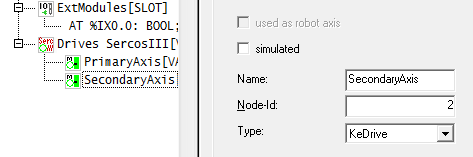
\includegraphics[width=9 cm]{images/DriveConfiguration} 
    \caption{Basiskonfiguration des sekundären Motors}
  \end{minipage}
\end{figure}

\subsubsection{Der Motion Task}
Der "'Motion Task"' dient dazu die Winkelstellungen der Motoren zu aktualisieren, hierzu wird in vom System vorgegebenen Abständen das Programm \textit{McMain} aufgerufen. Das genannte Hauptprogramm überprüft zuerst ob alle zur initialisierung notwendigen Schritte getätigt wurden und geht dann dazu über zuerst die aktuellen Winkelstellungen auszulesen, neue Soll-Werte zu setzen und diese Schließlich an die Motorsteuerungen weiterzugeben. 

Das setzen der neuen Winkelstellungen, sowie alle anderen Operation die eine Veränderung des Zustands der Motoren mit sich bringen passiert im Programm \textit{UserUpdate} welches zwischen dem Lesen der Ist-Werte und dem schreiben der Soll-Werte aufgerufen wird.

\subsubsection{Das UserUpdate Programm}
Das \textit{UserUpdate} Programm dient wie bereits erwähnt zum verändern des Zustands der Motoren. Das Programm ähnelt im Aufbau dem \textit{NetworkManager} Programm sehr stark da es ebenfalls über eine \textit{Switch} Kontrollstruktur gesteuert wird. Für eine genauere Beschreibung dieser Art von Programmaufbau siehe Unterkapitel "'Aufbau"' im Kapitel "'Die Netzwerkkommunikation"'.

Im initialen Status (\textit{state} = 0) beginnt das \textit{UserUpdate} Programm zuerst damit die einzelnen Motoren zu "'resetten"', dies ist notwendig um etwaige Fehler oder unbrauchbare Einstellungen aus der Motorsteuerung zu löschen. Die Operationen an den Motoren werden jeweils über vom System bereitgestellte Funktionsblöcke durchgeführt, welche zur richtigen Zeit mit den entsprechenden Parametern aufgerufen werden. Meist verfügt ein für eine Operation nötiger Funktionsblock über einen \textit{Execute} Parameter, welcher eine positive Flanke aufweisen muss damit die Operation durchgeführt wird. Aus diesem Grund ist es nötig die Funktionsblöcke zweimal aufzurufen, am Beispiel der "'reset"' Operation sieht dies folgendermaßen aus:
\begin{lstlisting}[language = codesysls, captionpos=b, caption={Resetten einer Motors}]
fb_reset_primaryAxis(Axis := SecondaryAxis, Execute := FALSE);
fb_reset_primaryAxis(Axis := SecondaryAxis, Execute := TRUE);
\end{lstlisting}

Nachdem dieser Schritt ausgeführt wurde, wird \textit{state} auf 1 gesetzt. 

Befindet sich das Programm im Status 1, so wird zuerst überprüft ob das "'resetten"' der Motorsteuerungen abgeschlossen ist. Ist dies der Fall, so wird der Funktionsblock für das "'resetten"' erneut aufgerufen um dem \textit{Execute} Parameter den Wert \textit{FALSE} zuzuweisen und damit den Motor für weitere Operationen freizugeben.
Nach Abschluss dieser Operation wird die \textit{state} Variable des Programms auf 10 gesetzt um beim nächsten Programmaufruf die Motoren einzuschalten.

Der nächste Schritt im Programm ist das Einschalten der Motoren, dies geschieht wieder über Aufruf des entsprechenden Funktionsblocks (\textit{MC\_Power}, muss zuvor instanziert worden sein). War das Einschalten der Motoren erfolgreich, so wechselt das Programm in den Status 12.

Im Status 12 überprüft das \textit{UserUpdate} Programm ob ein "'Homing"' also eine Suche nach der Ausgangsposition durchgeführt werden muss. Diese Überprüfung findet mithilfe der globalen Variable \textit{robot\_homing} stattd die gegebenenfalls durch das \textit{NetworkManager} Programm auf den Wert \textit{true} gesetzt wurde.
Da im Rahmen dieses Projektes keine Mechanik erstellt wurde, war das eigentliche "'Homing"' nicht implementierbar und es wird hier Fall lediglich die globale Variable \textit{robot\_homing} auf \textit{false} gesetzt. Zusätzlich wird die globale Variable \textit{robot\_ready} auf \textit{true} gesetzt um dem \textit{NetworkManager} Programm zu signalisieren dass der Roboter bereit ist Befehle zu empfangen. Das \textit{NetworkManager} Programm gibt diese Information an den Computer weiter. Am Ende wird die \textit{state} Variable auf 20 gesetzt.

Hat die \textit{state} Variable den Wert 20, so wartet der "'Motion Task"' auf neue Interpolationspunkte in Form von Winkelstellungen. Werden neue Interpolationspunkte durch das \textit{NetworkManager} Programm eingelesen, so werden sie in globale Array gespeichert, siehe Unterkapitel "'Ablauf des Datenempfanngs"' im Kapitel "'Netzwerkkommunikation"'. Wenn alle Werte fertig eingelesen wurden, wird die globale Variable \textit{stepsAvailable} auf die Länge des Array gesetzt. Hat die genannte Variable nun einen Wert der höher als 0 ist, so wird der erste Winkel aus dem Array an die Motorsteuerung als relativ zu verfahrender Winkel weitergegeben. Die Variable \textit{stepsAvailable} wird nun um 1 verringert und die Variable \textit{curStepIndex} wird um 1 erhöht. Die genannte \textit{curStepIndex} Variable ist zu Anfang 0 und dient dazu zu speichern welcher Schritt aus dem Array beim nächsten Aufruf des \textit{UserUpdate} Programms gefahren werden soll.
\begin{lstlisting}[language = codesysls, captionpos=b, caption={Übergabe der Winkel an die Motoren}]
20: (* Start relative Movement *)

		IF(stepsAvailable > 0)THEN

		fb_moveRelative_primaryAxis(Axis := PrimaryAxis, Execute := FALSE);
		fb_moveRelative_primaryAxis(Axis := PrimaryAxis, Execute := TRUE, Distance := primarySteps[currentStepIndex], Velocity := 300, Acceleration := 10000, Deceleration := 10000);

		fb_moveRelative_secondaryAxis(Axis := SecondaryAxis, Execute := FALSE);
		fb_moveRelative_secondaryAxis(Axis := SecondaryAxis, Execute := TRUE, Distance := primarySteps[currentStepIndex], Velocity := 300, Acceleration := 10000, Deceleration := 10000);

		currentStepIndex := currentStepIndex +1;
		stepsAvailable := stepsAvailable -1;
		END_IF;
\end{lstlisting}

Wurden alle Schritte gefahren, so wird die Variable \textit{robot\_ready} auf true gesetzt. 

Wird im Status 20 durch Kontrolle der \textit{robot\_shutdown} Variable erkannt dass der Roboter heruntergefahren werden soll, so wird \textit{state} auf 100 gesetzt. Damit werden beim nächsten Aufruf des Programms die  Motoren abgeschaltet.






\subsection{Konstruktion des Modells}
\subsubsection{Allgemein}
Im Rahmen dieses Projektes wurden bereits umfangreiche Überlegungen angestellt, wie ein stabileres, leistungsstärkeres Modell unter Verwendung der größeren Motoren der Firma KEBA verwirklicht werden könnte.
Grundsätzlich basierten alle Überlegungen bezüglich der Konstruktion dieses Modells auf einer Fertigung aus Aluminium. Hierfür wurden im Projektverlauf die entsprechenden Aluminiumprofile beschafft, welche später beim Bau noch auf die optimale Länge zurecht geschnitten werden müssen. 
Im Zuge dieser Überlegungen wurde auch ein Aluminiumrohling in Form einer 16 mm Dicken Platte beschafft aus dem die Teile des Gelenks gefräst werden sollen.

\subsubsection{Gelenke}
Einen Knackpunkt bei der Konstruktion des Aluminiummodells stellte der Aufbau der einzelnen Gelenke dar. Die schlussendlich gewählte Herangehensweise wurde bereits in dieser Diplomarbeit im Kapitel "'Komponenten des Edubot Modells"' beschrieben. Grundgedanke der Gelenke ist die Erzeugung eines Bauteils der grob gesagt aussieht wie ein liegendes U. In den beiden Längsseiten des Us befinden sich Kugellager durch welche eine Verlängerung der Motorwelle führt. 
An diese Wellenverlängerung wird dann der eigentliche Arm befestigt. Durch diese Konstruktionsweise werden alle Kräfte die durch das Gewicht des Armes entstehen durch die Kugellager getragen und haben keinen Einfluss auf die Laufeigenschaften des Motors.

\subsection{CNC Programmierung}
Die einzelnen Bauteile die zum Bau der im vorherigen Unterkapitel beschriebenen U-Förmigen Gelenke nötig sind wurden im Rahmen dieses Projektes als CNC Programm geschrieben und liegen dieser Arbeit bei. Als Werkzeug für die Erstellung der CNC Programme wurde die Software WinNC der Firma EMCO verwendet, welche in weiterer Folge auch für die Ausführung der Programme auf der schuleigenen Fräse verwendet werden kann. 
Grundsätzlich sind beim schreiben eines CNC Programmes nur die durch die Fräse auszuführenden Bewegungen und die jeweils benötigten Werkzeugoperationen aufzulisten. Für spezielle Operationen, wie beispielsweise das Fräsen einer Tasche oder das Bohren eines Gewindes stehen bereits vorgefertigte Operationen zur Verfügung die mit den richtigen Parametern aufgerufen werden müssen.
Leider gab es bei der Verwendung der WinNC Software Probleme mit der Lizenz, so dass zum Zeitpunkt der Anfertigung dieser schriftlichen Arbeit eine Simulation der CNC Programme nicht möglich war. Aus diesem Grund können hier keine Abbildungen gezeigt werden um die Einzelnen Bauteile zu präsentieren. Die Folgende Abbildung zeigt jedoch den einen Ausschnitt aus dem CNC Programm dass zur Erstellung eines Seitenteils des Gelenks verwendet werden kann, der gezeigte Ausschnitt dient dazu, Taschen für die Kugellager zu fräsen.

\begin{figure}[H]
\centering
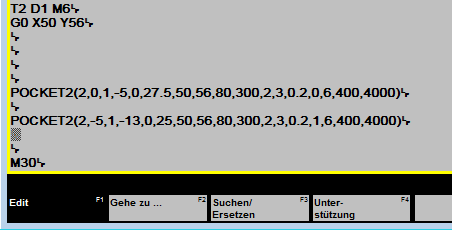
\includegraphics[width=9cm]{images/cncprogramm}
\caption{Screenshot eines CNC Programms in WinNC}
\end{figure}

\subsection{Sonstige Überlegungen}
Während der Planung der Mechanik des größeren Modells kamen wir unter Anderem zu dem Schluss, dass die Motoren nicht direkt mit den Armen verbunden werden sollten, sondern dass hier als Zwischenglied eine Übersetzung von Vorteil wäre. Diese Feststellung resultiert vor allem aus der Tatsache, dass die verwendeten Motoren sehr hohe Drehzahlen erreichen können und ihr maximaler Drehmoment im Gegenzug sehr begrenzt ist.


	\newpage
	
\label{chap:keba}

\section{Komponenten des KEBA Modells}


\subsection{Allgemein}            
Der Name Edubot bezeichnet sowohl das Softwaresystem als ganzes, als auch den aus Holz gefertigten Roboterarm. Der Roboterarm wird um Missverständnisse zu vermeiden allgemein als "'Edubot Modell"' bezeichnet. Es handelt sich bei diesem Roboterarm um eine Konstruktion mit zwei rotatorischen Achsen die so konzipiert wurde dass eine Erweiterung um diverse Werkzeuge oder weitere Achsen ohne Probleme und mit Hilfe des Handbuchs möglich ist. 

\begin{figure}[H]
  \centering
  \begin{minipage}[t]{12 cm}
  	\centering
  	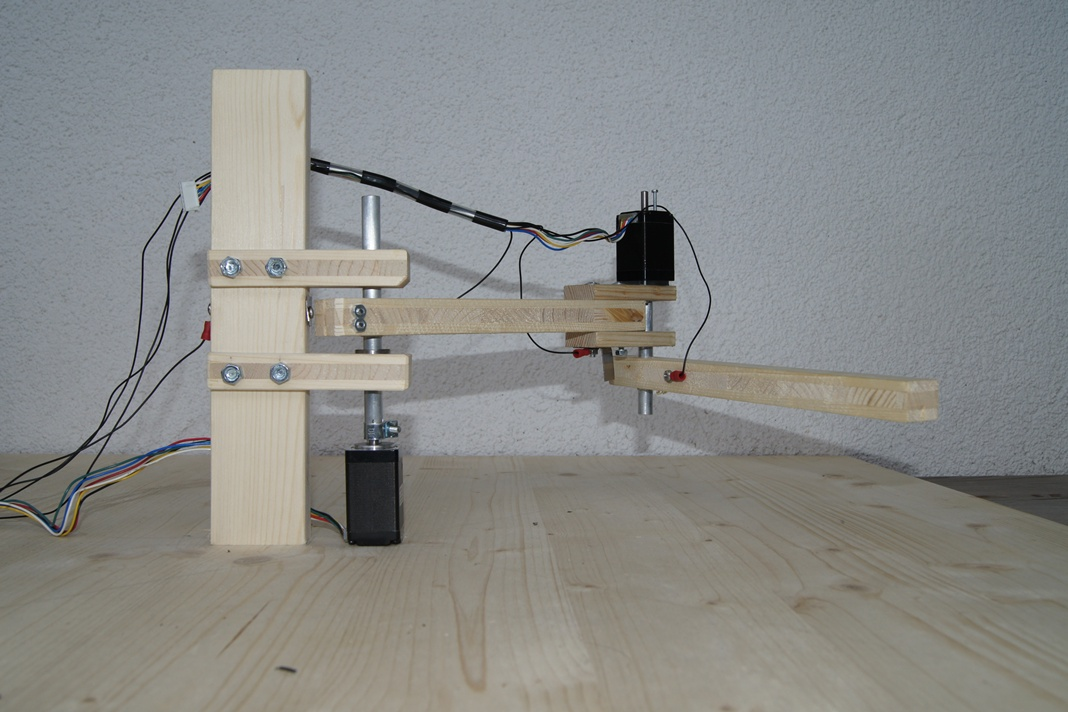
\includegraphics[width=12cm]{images/edubot_photo} 
    \caption{Das Edubot Modell}
  \end{minipage}
\end{figure}

\subsubsection{Aufgaben}
Das Edubot Modell soll als Anschauungsmaterial sowohl für den Unterricht, als für Anlässe wie den Tag der offenen Tür oder sonstige Präsentationszwecke dienen. Der Aufbau des Modells und die verwendete Elektronik wurde bewusst so simpel wie möglich gehalten um es Schülern zu ermöglichen schnell einen Überblick über die Funktionsweise und konstruktionstechnischen Eigenheiten zu erlangen.

\subsubsection{Funktionen}
Das Edubot Vorführmodell verfügt über zwei rotatorische Achsen die auf horizontaler Ebene bewegt werden können. 
Der Roboter besitzt damit zwei Freiheitsgrade und kann auf einer Ebene alle Punkte in einem Nieren-förmigen Arbeitsbereich anfahren. Abhängig vom montierten Werkzeug kann der Roboter beispielsweise dafür verwendet werden einfache Zeichnungen anzufertigen. Ein entsprechendes Werkzeug wird jedoch nicht mitgeliefert und muss selbst konstruiert werden.

\subsubsection{Bedienung}
Als Steuerungsteil des Roboterarms dient ein Mikrocontroller (GHI Embedded Master) welcher sowohl über eine Netzwerkschnittstelle, als auch über einen USB Anschluss verfügt. Zur Übergabe von Befehlen an den Roboter wird ausschließlich die Netzwerkschnittstelle verwendet. Der USB Anschluss  wird nur benötigt um Softwareänderungen am Controller durchzuführen.
Um dem Roboterarm Befehle zu übergeben, muss der Mikrocontroller mithilfe eines normalen Netzwerkkabels mit RJ-45 Steckern an einen Computer angeschlossen werden auf welchem eine Applikation läuft welche auf der mitgelieferten API aufbaut.

\subsection{Motoren}
Als Motoren wurden bei der Planung dieses Modells jene Drehstrom-Servomotoren verwendet die der Schule von der Firma Keba zur Verfügung gestellt wurden. 

Zum Betrieb der Motoren werden, ebenfalls in der Schule vorhandene, passende Motoransteuerungen benötigt. Für jeden Motor ist eine Steuerung nötig. 

Die Steuerungen werden über eine SercosII Schnittstelle mit der SPS verbunden. Die Verbindung erfolgt über normale Patch Kabel, eine Steuerung wird direkt mit der SPS verbunden, die zweite wird dann mit dieser ersten Steuerung verbunden. Über den kleinen Display an der Motorsteuerung lassen sich die benötigten Einstellungen bezüglich der Rolle die der angeschlossene Motor spielt tätigen und es muss zur einzelnen Ansteuerung jedem Motor eine Nummer gegeben werden.

\subsection{Netzwerkschnittstelle}
\subsubsection{Allgemein}
Die Netzwerkschnittstelle des KEBA Modells ist auf der SPS implementiert und soll die Kommunikation mit der Roboter API ermöglichen, diese Kommunikation verläuft über Sockets und unterscheidet sich im Prinzip wenig von jener auf dem Edubot Modell, lediglich die Art der Implementierung unterscheidet sich auf Grund der unterschiedlichen Programmierumgebungen sehr stark. Für die implentierung der Netzwerkfunktionalität wurde die frei zur Verfügung stehende OSCAT Library verwendet, welche im Kapitel "'Verwendete Technologien und Werkzeuge"' kurz erklärt wird. 

Die Netzwerkschnittstelle ist sowohl für den Empang von Befehlen und Pfaden, als auch für die Rückgabe von Statusinformationen verantwortlich und ist auf der SPS als Aufgabe ohne harte Echtzeitanforderungen definiert, da keine Hardware direkt angesteuert wird und es dadurch nicht nötig ist zu einem genau bestimmten Zeitpunkt zu arbeiten.

\subsubsection{Aufbau}
Die Netzwerkschnittstelle ist im Programm \textit{NetworkManager} implementiert und wird durch einen Entsprechenden "'Task"' in zyklischen Abständen von 200ms aufgerufen. Da nicht bei jedem Programmaufruf sämtliche Operationen wie beispielsweise die Initialisierung der für den Empfang benötigten Variablen vorgenommen werden sollen, sondern vielmehr abhängig vom aktuellen Status der Kommunikation unterschiedliche Programmteile benötigt werden, basieren zyklisch aufgerufenen Programmen meist auf einer \textit{Switch} Kontrollstruktur. Die \textit{Switch} Kontrollstruktor entscheidet mittels einer \textit{status} Variable, welche Operationen derzeit benötigt werden. In den einzelnen Fällen der \textit{Switch} Struktur befindet sich die Programmlogik die Ausgeführt werden soll wenn die \textit{status} Variable den Wert dieses Falles annimmt. Üblicherweise ist der ist der Anfangswert der \textit{status} Variable 0, wodurch beim ersten zyklischen Aufruf des Programms die dem Fall 0 zugeordnete Programmlogik ausgeführt wird. Diese Programmlogik kann beispielsweise zur Initialisierung von Variablen dienen. Wurde die Inititialisiierung, um kurz an diesem Beispiel festzuhalten, erfolgreich beendet, so wird im Fall 0 noch die \textit{status} Variable so gesetzt, dass beim nächsten Programmaufruf die nach der initialisierung auszuführende Programmlogik ausgeführt wird. Dieses Prinzip kann nun innerhalb des Programms beliebig fortgeführt werden.

\subsubsection{Umsetzung}
Auf die genau Implementierung der Netzwerkkommunikation auf der SPS wird hier nur oberflächlich eingegangen, genauere Informationen hierzu sind der Dokumentation der OSCAT Network Library und dem Source Code der SPS zu entnehmen, welcher im Rahmen der Diplomarbeit gemeinsam mit der restlichen Software des Edubot Systems abgegeben wurde. Im Folgenden erfolgt lediglich eine Kurze Aufzählung der wichtigsten Objekte und ihrer Verwendung:
\begin{itemize}
\item \textbf{IP\_CONTROL}\\
Der Typ IP\_CONTROL ist der zentrale Baustein einer Netzwerkkommunikation mit OSCAT. Über ein Objekt dieses Typs werden alle wichtigen Operationen zur Komunikation, wie beispielsweise das anlegen eines Sockets und das Empfangen der Daten abgewickelt. Zum Verbindungsaufbau über ein IP\_CONTROL Objekt ist es lediglich Nötig, dieses mit den entsprechenden Parametern anzulegen und in periodischen Abständen zu Überprüfen ob bereits eine Verbindung hergestellt wurde, dies geschieht über das state Attribut des IP\_CONTROL Objekts, welches jederzeit den Verbindungsstatus in Form eines Integer Wertes beinhaltet, die möglichen Werte dieses Attributs sind der OSCAT Network Library Dokumentation zu entnehmen

\item \textbf{IP\_C}\\
Zur Erzeugung eines IP\_CONTROL Objekts muss ein IP\_C Objekt übergeben werden, welches alle nötigen Parameter für die Verbindung enthält. Zwar verfügt das IP\_CONTROL selbst bereits über einige entsprechende Attribute, diese sollten jedoch nur als default Werte verwendet und von denen im IP\_C Objekt überschrieben werden. 
Wichtige Attribute eines IP\_C Objekts sind zum Beispiel C\_MODE, welches angibt welche Art der Verbindung aufgebaut werden soll, C\_ENABLE zum freigeben der Verbindung und R\_OBSERVE zur Aktivierung des Dateiempfangs.

\item \textbf{NETWORK\_BUFFER}\\
Bei der Erzeugung eines IP\_CONTROL Objekts muss um das Senden beziehungsweise Empfangen von Nachrichten zu ermöglichen je ein Objekt vom Typ NETWORK\_BUFFER als Lesebuffer und eines als Schreibbuffer mitgegeben werden. Ein Objekt vom Typ NETWORK\_BUFFER ist grundsätzlich dazu da entweder empfangene Daten zu einem Stream zu Sammeln um sie später komfortabel auslesen zu können oder zu sendende Daten für die Netzwerkübertragung aufzubereiten um sie später als den zulässigen Blockgrößen entsprechende Pakete zu versenden.
\end{itemize}

\subsubsection{Ablauf des Datenempfanngs}

Um eine Netzwerkverbindung herzustellen muss zuerst ein IP\_C Objekt zur Speicherung der Verbindungsparameter (siehe Kapitel "'Umsetzung"') angelegt werden.
Ebenfalls vor Beginn der Kommunikation müssen zwei NETWORK\_BUFFER Objekte für das Senden und Empfangen von Daten angelegt und initialisiert werden. 
Wie bereits im Kapitel "'Aufbau"' beschrieben, basiert die Netzwerkkomunikation auf einem zyklisch aufgerufenen Programm, welches über einen \textit{Integer} Variable die aktuell auszuführende Operation definiert. Die eben beschriebenen Operationen sollen am Anfang des Programms und somit wenn die \textit {state} Variable auf ihren Initialwert 0 gesetzt ist ausgeführt werden. Nach der Ausführung dieser Schritte wird \textit {state} so gesetzt dass beim nächsten Programmaufruf der nächste Schritt ausgführt wird, in unserem Fall wird \textit{state} auf 10 gesetzt.

Als nächster Schritt (\textit{state} = 10) muss nun ein  IP\_CONTROL aufgerufen werden. Die vorher instanzierten Objekte hierbei werden direkt übergeben. Durch diesen Schritt beginnt die SPS auf eingehende Verbindungen zu horchen.
Ein Beispiel für den Aufruf des IP\_CONTROL's sieht folgendermaßen aus:

IP\_CONTROL1(PORT:=400 ,TIME\_OUT:=T\#1s,IP\_C:= IP\_C1,S\_BUF:=S\_BUF1, R\_BUF:=R\_BUF1 );

Durch regelmäßiges überprüfen des \textit{state} Attributs des IP\_CONTROL Objektes kann nun festgestellt werden wenn eine neue Verbindung hergestellt wurde. Bekommt das \textit{state} Attribut des IP\_CONTROLs den Wert 254, so wurde die Verbindung erfolgreich aufgebaut und es kann zum Datenempfang übergegangen werden. Hierzu wird die \textit{state} Variable des Programms auf 30 gesetzt.

Während des Wartens auf Dateiempfang (\textit{state} = 30) wird in regelmäßigen Abständen das \textit{size} Attribut des dem IP\_CONTROLL mitgegebenen NETWORK\_BUFFER Objekts - im obigen Beispielfall R\_BUF1 - überprüft. Nimmt das \textit{size} Attribut einen Wert an der höher als 0 ist, so wurden Daten empfangen und können aus dem NETWORK\_BUFFER ausgelesen werden. Der NETWORK\_BUFFER enthält hierzu ein array aus \textit{byte} Werten welches werden kann. Die einzelnen Byte Werte werden mithilfe einer einfachen selbst geschriebenen Funktion (siehe BYTE\_TO\_CHAR Funktion im Kapitel "'Hilfsfunktionen"') in eine Zeichenkette umgewandelt. Die \textit{state} Variable wird dannach auf den Wert 40 gesetzt um im nächsten Programmdurchlauf die empfangene Zeichenkette zu analysieren.

Liegt die übertragene Nachricht als Zeichenkette vom Typ \textit{string} vor (\textit{state = 40}), so werden zuerst ihre ersten drei Buchstaben überprüft. Diese drei Buchchstaben enthalten, ähnlich wie beim Edubot Modell, die Information welche Operation ausgeführt werden soll. 
Abhängig von der zu tätigenden Operation werden nun globale Variablen verändert, Daten konvertiert. Die folgende Auflistung gibt an welche Aktionen bei Empfang der wichtigsten Befehle ausgeführt werden:

\begin{itemize}
\item \textbf{Befehl "mvs"}\\
Der Befehl informiert die Steuerung darüber, dass eine lineare Bewegung ausgeführt werden soll. Enthält die Empfangene Zeichenkette diesen Befehl in ihren ersten drei Zeichen, so enthält der rest der Zeichenkette alle zum Abfahren dieser Bewegung benötigten Punkte.
Mit Hilfe einer weiteren selbst geschriebenen Funktion (siehe "'InterpretToGlobalStepArray"' Funktion im nächsten Kapitel "'Hilfsfunktionen"') wirden die in der Zeicehnkette enthaltenen Interpolationspunkte in Arrays vom Typ Real (Gleitkommadatentyp) umgewandelt und als globale Variablen abgelegt. Hierbei wird für jede Achse ein Array angelegt das für jeden Intapolationsschritt den richtigen Winkel angiebt. Aus diesem Array liest später der für die Bewegung zuständige "'MotionTask"' die aktuell zu verfahrenden Winkel aus und übergiebt sie an die Motorsteuerung um die Bewegung phsysisch durchzuführen. Dieser Vorgang ist im Unterkapitel "'Steuerung der Motoren"'' genauer erklärt. Zusätz
\item \textbf{Befehl "hom"}\\
Enthält die empfangene Zeichenkette als Präfix die Zeichen "hom", so wird der Steuerung bekannt gegeben dass der Roboter seine Ausgangsposition suchen soll. Da zum aktuellen Zeitpunkt keine Hardware zur Verfügung stand konnte dieser Vorgang nicht implementiert werden und es wird hier lediglich ein globaler \textit{boolean} Wert auf \textit{true} gesetzt welche später "'MotionTask"' den "'Homing Prozess" auslösen soll.'
\item \textbf{Befehl "sht"}\\
Der Befehl "sht" dient dazu den Roboter auszuschalten, also alle Motoren zu deaktivieren und sonstige zum herunterfahren nötige Abläufe durchzuführen. 
\end{itemize}

\subsubsection{Hilfsfunktionen}
Um diverse Umrechnungen zu vereinfachen und redundaten Programmcode zu vermeiden wurden diverse Hilfsunktionen erzeugt die an enprechnder Stelle im\textit{ NetworkManager} Programm verwendet werden, die folgende Auflistung soll einen Überblick über diese Funktionen bieten, Informationen über ihre Funktionalität bereitstellen und ihre Verwendung im Programm kurz beschreiben:

\begin{itemize}
\item \textbf{BYTE\_TO\_CHAR}\\
Da von CoDeSys standardmäßig keine Funktion zur umrechnung eines \textit{byte} Wertes in einen \textit{char} Wert zur Verfügung gestellt wird, diese aber für die Umrechnung des empfangenen \textit{byte} Arrays in einen String benötigt wird, musste eine entsprechende Funktion selbst erzeugt werden. Die beschriebene Funktion erhält als input Parameter einen einzelnen \textit{byte} Wert und gibt einen Einstelligen \textit{string} Wert zurück, welcher als Inhalt den umgerrechneten \textit{byte} Wert enthält. Das \textit{NetwokManager} Programm ruft diese Funktion innerhalb einer Schleife auf welcher das empfangene \textit{byte} Array mit Hilfe einer Schleife durchläuft und die Ergebnisse der Umrechnung zu einem einzigen String zusammenfügt.

\item \textbf{CHAR\_TO\_BYTE}\\
Diese Funktion bildet das Gegenstückk zur im letzten Schritt beschriebenen Methode, sie wandelt einzelne \textit{char} Werte in Bytes um. Dies ist notwendig um im \textit{NetwokManager} Programm den an den Computer zu sendenden, als \textit{string} vorliegeneden Status  in ein sendbares \textit{byte} Array umzuwandeln, auch hier kommt wieder eine Schleife zur einzelnen Umwandlung aller im \textit{string} enthaltenen Zeichen zum Einsatz.

\item \textbf{InterpretToGlobalStepArray}\\
Da die Empfangenen Schrittinformation in Form einer Zeichenkette nicht direkt vom "'Motion Task" verwendet werden kann, ist es notwendig diese vorher in einzelne Arrays für jeden Motor zu zerlegen. Hierzu wird der Funktion \textit{InterpretToGlobalStepArray} die zu konvertierende Zeichenkette übergeben. In der Funktion selbst wird die Zeichenkette wiederum in einzelne Zeichenketten zerlegt die jeweils die zu verfahrenden Winkel für einen einzelnen Schritt pro Motor angeben. Diese Zeichenkette wird zur Umwandlung der Winkelstellungen in Werte vom Typ \textit{real} der Hilfsfunktion \textit{InterpretToAngles} überbeben. Das von der genannten Funktion zurückgegebene Array enthält nun gewünschten Winkel in Werten vom Typ \textit{real}. Diese Werte werden nun in die globalen Array der einzelnen Motoren angefügt. Nach Umwandlung aller Werte wird schließlich die globale Variable \textit{stepsAvailable} auf die Anzahl der konvertierten Schritte gesetzt. Zusätzlich wird die globale Variable \textit{robot\_ready} auf \textit{false} gesetzt.

\item \textbf{InterpretToAngles}\\
Diese Funktion dienst dazu, die in Form einer Zeichenkette als Parameter übergebenen Winkel eines einzelnen Interpolationsschrittes in ein Array vom Typ \textit{real} umzuwandeln und zurückzugeben.

\end{itemize}

\subsubsection{Der Rückmelde-Prozess}
Wurden der Datenempfang und alle im \textit{NetworkManager} durchzuführenden Operation zur ordnungsgemäßen Abarbeitung der Befehle abgeschlossen, so wird wie im Kapitel "'Ablauf des Dateiempfang"' bereits erwähnt, die \textit{state} Variable des Programms auf 110 gesetzt. Befindet sich das Programm in diesem Zustand, so werden bei jedem Aufruf globale Statusvariablen überprüft um bei bestimmten Veränderungen eine entsprechende Rückmmeldung an den Verbundenen Computer zu geben. Die wichtigsten Variablen sind hierbei \textit{robot\_ready}, \textit{robot\_shutdown} und \textit{robot\_failure}.

Ist die \textit{robot\_ready} Variable auf \textit{true} gesetzt, so sendet das \textit{NetworkManager} wird zuerst eine Zeichenkette mit dem Wert "'ready"' erzeugt, mithilfe einer Schleife und der der Hilfsfunktion CHAR\_TO\_BYTE in einzelne Bytes zerlegt und dem zum Senden vorgesehenen NETWORK\_BUFFER Objekt übergeben. In unserem Fall trägt dieses Objekt den Namen "'S\_BUFF1"'. Nun kann durch Aufruf des IP\_CONTROLLs die Zeichenkette an den Computer übergeben werden um zu signalisieren dass der Roboter bereit ist neue Befehle zum empfangen. Nach Beendigung der Übertragung wird die \textit{state} Variable des Programms auf den Wert 30 gesetzt um beim nächsten Aufruf wieder auf Daten zu horchen.

Befinden sich hingegen entweder die globale Variable \textit{robot\_shutdown} oder \textit{robot\_failure} im Status \textit{true}, so wird die Zeichenkette "'shutdown"' in konvertiert und dem Sendebuffer übergeben. Damit wird dem Computer mitgeteilt dass der Roboter derzeit nicht verwendbar ist und entweder heruntergefahren wurde oder ein Fehler aufgetreten ist. In beiden Fällen muss eine neue Verbindung mit der Steuerung hergestellt werden und somit der "'Homing Prozess"' durchgeführt werden. Nach dem Senden dieser Mitteilung wird die Verbindung beendet und die \textit{state} Variable wird auf 0 gesetzt um das \textit{NetworkManager} Programm neu zu initialisieren. 

Um die Verbindung zu beenden muss Aufgrund eines Fehler in der OSCAT Library zuerst der Socket manuell geschlossen werden, dies passiert am Beispiel der Steuerungssoftware mit folgender Zeile:

SysSockClose(diSocket:=IP\_CONTROL1.socket);

Wurde dieser Schritt ausgeführt kann über das C\_ENABLED Attribut des übergebenen IP\_C Objekts das IP\_CONTROL abgeschaltet werden.




\subsection{Motoransteuerung}
Diese Kapitel behandelt Programmvorgänge die in der SPS nötig sind, um die Motoren mit eine korrekte Bahn fahren zu lassen. Welche Voraussetzungen aus Sicht der Hardware gegeben sein müssen ist dem Kapitel "'Motoren"' zu entnehmen.

\subsubsection{Vorgehensweise}
Anfangs war geplant für die Steuerung der Motoren die internen Interpolationsfunktionen der KEBA Steuerung zu verwenden, welche im Rahmen des Zusatzsystems KeMotion zur Verfügung gestellt werden. KeMotion ist eine Softwarekomponente die für KEBA Steuerungen angeboten wird und umfangreiche Funktionen zum Betrieb von Industrierobotern zur Verfügung stellt.
Leider ist das KeMotion System dafür ausgelegt Pfadinformationen in Form von Vorgefertigten Dateien des Dateityps KAIRO zu Verarbeiten. Es ist vorgesehen dass diese Dateien, welche die anzufahrenden Punkte in Form einer einfachen Scriptsprache (ähnlich einer CNC Programmiersprache) enthalten, bereits beim Programmstart vorhanden sind oder mithilfe eines geeigneten Teach-In Geräts (Gerät zur Eingabe der Bahn) erzeugt werden. Diese Eigenheit bereitete unverhältnismäßig große Schwierigkeiten da im Edubot-System die Punkte über die Netzwerkschnittstelle übergeben werden und so erst zur Laufzeit auf das Gerät gelangen. 
Aus diesem Grund und basierend auf der Tatsache dass die Edubot API ebenfalls über funktionstüchtige Mechanismen für Bahninterpolation und Invers-Kinematik verfügt, fiel der Entschluss, ähnlich wie beim Edubot Modell bereits fertig interpolierte Bahnen in Form einer Liste an Punkten zu übergeben. Ein Vorteil dieser Vorgehensweise ist die bessere Überschaubarkeit der Steuerungssoftware, wodurch die Möglichkeit gegeben ist sie optimal für Schulungszwecke einzusetzen.

\subsubsection{Basiseinstellungen}
Um die Ansteuerung der Motoren grundsätzlich zu ermöglichen, ist es nötig im Menüpunkt "'PLC Configuration"' in KeStudio einen neuen Knotenpunkt anzulegen. Dieser Knotenpunkt ist vom Typ "'Drives SercosIII"' und dient als übergeordnetes Element für alle über die SercosIII Schnittstelle angeschlossenen Motoren. 
Es können nun neue Unterelemente für den angelegten Knotenpunkt erzeugt werden. Diese Unterpunkte haben den Typ "'Drive SercosIII"' und repräsentieren jeweils einen einzelnen Motor. Es muss nun noch jedem Motor ein entsprechender Name gegeben werden über den er später aus dem Programmcode ansprechbar sein soll. Zusätzlich muss für die einzelnen Motoren jeweils die "'Node-ID"' angegeben werden, also jene Nummer die auf der Steuerung des Motors unter dem Menüpunkt "'Slave"' festgelegt wurde.

\begin{figure}[H]
  \centering
  \begin{minipage}[t]{9 cm}
  	\centering
  	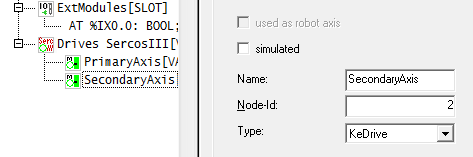
\includegraphics[width=9 cm]{images/DriveConfiguration} 
    \caption{Basiskonfiguration des sekundären Motors}
  \end{minipage}
\end{figure}

\subsubsection{Der Motion Task}
Der "'Motion Task"' dient dazu die Winkelstellungen der Motoren zu aktualisieren, hierzu wird in vom System vorgegebenen Abständen das Programm \textit{McMain} aufgerufen. Das genannte Hauptprogramm überprüft zuerst ob alle zur initialisierung notwendigen Schritte getätigt wurden und geht dann dazu über zuerst die aktuellen Winkelstellungen auszulesen, neue Soll-Werte zu setzen und diese Schließlich an die Motorsteuerungen weiterzugeben. 

Das setzen der neuen Winkelstellungen, sowie alle anderen Operation die eine Veränderung des Zustands der Motoren mit sich bringen passiert im Programm \textit{UserUpdate} welches zwischen dem Lesen der Ist-Werte und dem schreiben der Soll-Werte aufgerufen wird.

\subsubsection{Das UserUpdate Programm}
Das \textit{UserUpdate} Programm dient wie bereits erwähnt zum verändern des Zustands der Motoren. Das Programm ähnelt im Aufbau dem \textit{NetworkManager} Programm sehr stark da es ebenfalls über eine \textit{Switch} Kontrollstruktur gesteuert wird. Für eine genauere Beschreibung dieser Art von Programmaufbau siehe Unterkapitel "'Aufbau"' im Kapitel "'Die Netzwerkkommunikation"'.

Im initialen Status (\textit{state} = 0) beginnt das \textit{UserUpdate} Programm zuerst damit die einzelnen Motoren zu "'resetten"', dies ist notwendig um etwaige Fehler oder unbrauchbare Einstellungen aus der Motorsteuerung zu löschen. Die Operationen an den Motoren werden jeweils über vom System bereitgestellte Funktionsblöcke durchgeführt, welche zur richtigen Zeit mit den entsprechenden Parametern aufgerufen werden. Meist verfügt ein für eine Operation nötiger Funktionsblock über einen \textit{Execute} Parameter, welcher eine positive Flanke aufweisen muss damit die Operation durchgeführt wird. Aus diesem Grund ist es nötig die Funktionsblöcke zweimal aufzurufen, am Beispiel der "'reset"' Operation sieht dies folgendermaßen aus:
\begin{lstlisting}[language = codesysls, captionpos=b, caption={Resetten einer Motors}]
fb_reset_primaryAxis(Axis := SecondaryAxis, Execute := FALSE);
fb_reset_primaryAxis(Axis := SecondaryAxis, Execute := TRUE);
\end{lstlisting}

Nachdem dieser Schritt ausgeführt wurde, wird \textit{state} auf 1 gesetzt. 

Befindet sich das Programm im Status 1, so wird zuerst überprüft ob das "'resetten"' der Motorsteuerungen abgeschlossen ist. Ist dies der Fall, so wird der Funktionsblock für das "'resetten"' erneut aufgerufen um dem \textit{Execute} Parameter den Wert \textit{FALSE} zuzuweisen und damit den Motor für weitere Operationen freizugeben.
Nach Abschluss dieser Operation wird die \textit{state} Variable des Programms auf 10 gesetzt um beim nächsten Programmaufruf die Motoren einzuschalten.

Der nächste Schritt im Programm ist das Einschalten der Motoren, dies geschieht wieder über Aufruf des entsprechenden Funktionsblocks (\textit{MC\_Power}, muss zuvor instanziert worden sein). War das Einschalten der Motoren erfolgreich, so wechselt das Programm in den Status 12.

Im Status 12 überprüft das \textit{UserUpdate} Programm ob ein "'Homing"' also eine Suche nach der Ausgangsposition durchgeführt werden muss. Diese Überprüfung findet mithilfe der globalen Variable \textit{robot\_homing} stattd die gegebenenfalls durch das \textit{NetworkManager} Programm auf den Wert \textit{true} gesetzt wurde.
Da im Rahmen dieses Projektes keine Mechanik erstellt wurde, war das eigentliche "'Homing"' nicht implementierbar und es wird hier Fall lediglich die globale Variable \textit{robot\_homing} auf \textit{false} gesetzt. Zusätzlich wird die globale Variable \textit{robot\_ready} auf \textit{true} gesetzt um dem \textit{NetworkManager} Programm zu signalisieren dass der Roboter bereit ist Befehle zu empfangen. Das \textit{NetworkManager} Programm gibt diese Information an den Computer weiter. Am Ende wird die \textit{state} Variable auf 20 gesetzt.

Hat die \textit{state} Variable den Wert 20, so wartet der "'Motion Task"' auf neue Interpolationspunkte in Form von Winkelstellungen. Werden neue Interpolationspunkte durch das \textit{NetworkManager} Programm eingelesen, so werden sie in globale Array gespeichert, siehe Unterkapitel "'Ablauf des Datenempfanngs"' im Kapitel "'Netzwerkkommunikation"'. Wenn alle Werte fertig eingelesen wurden, wird die globale Variable \textit{stepsAvailable} auf die Länge des Array gesetzt. Hat die genannte Variable nun einen Wert der höher als 0 ist, so wird der erste Winkel aus dem Array an die Motorsteuerung als relativ zu verfahrender Winkel weitergegeben. Die Variable \textit{stepsAvailable} wird nun um 1 verringert und die Variable \textit{curStepIndex} wird um 1 erhöht. Die genannte \textit{curStepIndex} Variable ist zu Anfang 0 und dient dazu zu speichern welcher Schritt aus dem Array beim nächsten Aufruf des \textit{UserUpdate} Programms gefahren werden soll.
\begin{lstlisting}[language = codesysls, captionpos=b, caption={Übergabe der Winkel an die Motoren}]
20: (* Start relative Movement *)

		IF(stepsAvailable > 0)THEN

		fb_moveRelative_primaryAxis(Axis := PrimaryAxis, Execute := FALSE);
		fb_moveRelative_primaryAxis(Axis := PrimaryAxis, Execute := TRUE, Distance := primarySteps[currentStepIndex], Velocity := 300, Acceleration := 10000, Deceleration := 10000);

		fb_moveRelative_secondaryAxis(Axis := SecondaryAxis, Execute := FALSE);
		fb_moveRelative_secondaryAxis(Axis := SecondaryAxis, Execute := TRUE, Distance := primarySteps[currentStepIndex], Velocity := 300, Acceleration := 10000, Deceleration := 10000);

		currentStepIndex := currentStepIndex +1;
		stepsAvailable := stepsAvailable -1;
		END_IF;
\end{lstlisting}

Wurden alle Schritte gefahren, so wird die Variable \textit{robot\_ready} auf true gesetzt. 

Wird im Status 20 durch Kontrolle der \textit{robot\_shutdown} Variable erkannt dass der Roboter heruntergefahren werden soll, so wird \textit{state} auf 100 gesetzt. Damit werden beim nächsten Aufruf des Programms die  Motoren abgeschaltet.






\subsection{Konstruktion des Modells}
\subsubsection{Allgemein}
Im Rahmen dieses Projektes wurden bereits umfangreiche Überlegungen angestellt, wie ein stabileres, leistungsstärkeres Modell unter Verwendung der größeren Motoren der Firma KEBA verwirklicht werden könnte.
Grundsätzlich basierten alle Überlegungen bezüglich der Konstruktion dieses Modells auf einer Fertigung aus Aluminium. Hierfür wurden im Projektverlauf die entsprechenden Aluminiumprofile beschafft, welche später beim Bau noch auf die optimale Länge zurecht geschnitten werden müssen. 
Im Zuge dieser Überlegungen wurde auch ein Aluminiumrohling in Form einer 16 mm Dicken Platte beschafft aus dem die Teile des Gelenks gefräst werden sollen.

\subsubsection{Gelenke}
Einen Knackpunkt bei der Konstruktion des Aluminiummodells stellte der Aufbau der einzelnen Gelenke dar. Die schlussendlich gewählte Herangehensweise wurde bereits in dieser Diplomarbeit im Kapitel "'Komponenten des Edubot Modells"' beschrieben. Grundgedanke der Gelenke ist die Erzeugung eines Bauteils der grob gesagt aussieht wie ein liegendes U. In den beiden Längsseiten des Us befinden sich Kugellager durch welche eine Verlängerung der Motorwelle führt. 
An diese Wellenverlängerung wird dann der eigentliche Arm befestigt. Durch diese Konstruktionsweise werden alle Kräfte die durch das Gewicht des Armes entstehen durch die Kugellager getragen und haben keinen Einfluss auf die Laufeigenschaften des Motors.

\subsection{CNC Programmierung}
Die einzelnen Bauteile die zum Bau der im vorherigen Unterkapitel beschriebenen U-Förmigen Gelenke nötig sind wurden im Rahmen dieses Projektes als CNC Programm geschrieben und liegen dieser Arbeit bei. Als Werkzeug für die Erstellung der CNC Programme wurde die Software WinNC der Firma EMCO verwendet, welche in weiterer Folge auch für die Ausführung der Programme auf der schuleigenen Fräse verwendet werden kann. 
Grundsätzlich sind beim schreiben eines CNC Programmes nur die durch die Fräse auszuführenden Bewegungen und die jeweils benötigten Werkzeugoperationen aufzulisten. Für spezielle Operationen, wie beispielsweise das Fräsen einer Tasche oder das Bohren eines Gewindes stehen bereits vorgefertigte Operationen zur Verfügung die mit den richtigen Parametern aufgerufen werden müssen.
Leider gab es bei der Verwendung der WinNC Software Probleme mit der Lizenz, so dass zum Zeitpunkt der Anfertigung dieser schriftlichen Arbeit eine Simulation der CNC Programme nicht möglich war. Aus diesem Grund können hier keine Abbildungen gezeigt werden um die Einzelnen Bauteile zu präsentieren. Die Folgende Abbildung zeigt jedoch den einen Ausschnitt aus dem CNC Programm dass zur Erstellung eines Seitenteils des Gelenks verwendet werden kann, der gezeigte Ausschnitt dient dazu, Taschen für die Kugellager zu fräsen.

\begin{figure}[H]
\centering
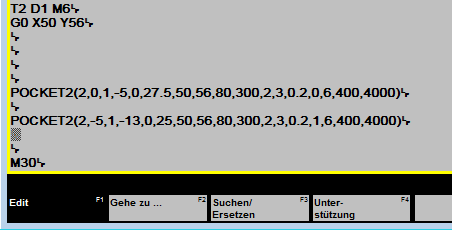
\includegraphics[width=9cm]{images/cncprogramm}
\caption{Screenshot eines CNC Programms in WinNC}
\end{figure}

\subsection{Sonstige Überlegungen}
Während der Planung der Mechanik des größeren Modells kamen wir unter Anderem zu dem Schluss, dass die Motoren nicht direkt mit den Armen verbunden werden sollten, sondern dass hier als Zwischenglied eine Übersetzung von Vorteil wäre. Diese Feststellung resultiert vor allem aus der Tatsache, dass die verwendeten Motoren sehr hohe Drehzahlen erreichen können und ihr maximaler Drehmoment im Gegenzug sehr begrenzt ist.


	
	
		
	%
  	% Bibliography
 	% 
	\newpage
	\fancyhead[L]{}
	\fancyhead[R]{}
	\renewcommand{\headrulewidth}{0.0pt}
	\fancyfoot[LO,RE]{\small \emph{Edubot}}
	\fancyfoot[RO,LE]{\small \thepage}
	\pagenumbering{Roman}
	\setcounter{page}{6}
	\phantomsection
	\addcontentsline{toc}{section}{Literatur}
	\printbibliography
\end{document}

%
% EoF
%
